%%%%%%%%%%%%%%%%%%%%%%%%%%%%%%%%%%%%%%%%%%%%%%%%%%%%%%%%%%%%%%%%%%%%%%%%%%%%%%%%
%									Chapter 4								   %
%%%%%%%%%%%%%%%%%%%%%%%%%%%%%%%%%%%%%%%%%%%%%%%%%%%%%%%%%%%%%%%%%%%%%%%%%%%%%%%%
\chapter{Deep Learning for Side-Channel Analysis}
\label{chap:machine_learning}
\citationChap{
	If someone can explain every phenomenon, his explanations are worthless.}{Shalev-Shwartz and Ben-David~\cite{shalev-shwartz_understanding_2014}
}
\minitoc
\newpage
%%%%%%%%%%%%%%%%%%%%%%%%%%%%%%%%%%%%%%%%%%%%%%%%%%%%%%%%%%%%%%%%%%%%%%%%%%%%%%%%
% Introduction
We have presented the \gls{sca} framework in \autoref{chap:sca}, and the profiling attacks in particular.
Indeed, the profiling phase in our considered attack scenario aims at leveraging the access to the traces measured on the clone device in order to improve the modelization of the leakage behavior of the target device.
We will see in this chapter that the latter process may be encompassed into the field of machine learning.
This chapter is devoted to introduce the necessary notions of this field to discuss the use of \gls{dl}-based \gls{sca} later in this thesis.

% Plan of this chapter
In \autoref{sec:theory_ml} we present the theoretical notions of \gls{ml}.
Then, \autoref{sec:dnns} and \autoref{sec:implementing_dnns} briefly recall the main principles of \gls{dl}, before we propose a review of its use in \gls{sca} in \autoref{sec:review_dl_sca}.
This will serve as a way to legitimate the outcomes of our research through this thesis in the next chapters.

\section{The Statistical Learning Theory}
    \label{sec:theory_ml}
    %%%%%%%%%%%%%%%%%%%%%%%%%%%%%%%%%%%%%%%%%%%%%%%%%%%%%%%%%%%%%%%%%%%%%%%%%%%%%%%%
%						MACHINE LEARNING THEORY					   			   %
%%%%%%%%%%%%%%%%%%%%%%%%%%%%%%%%%%%%%%%%%%%%%%%%%%%%%%%%%%%%%%%%%%%%%%%%%%%%%%%%
\subsection{Position of the Problem}
\label{sec:pb_position}
We stated in \autoref{sec:thm_heuser} that from an evaluator's point of view, it would be optimal to use the maximum likelihood distinguisher defined by \autoref{eq:mle_def}.
Unfortunately, it requires to know the true conditional \gls{pmf} \(\prob{\Z \given \XXX}\), which is unknown in practice.
Instead, the evaluator or the attacker can substitute the latter one with a model \(\MLmodel: \leakSpace \rightarrow \probSet{\sensVarSet}\), giving the following surrogate distinguisher:
\begin{equation}
	\MLMLEscore{\attackSet}{\MLmodel}[\key] = \sum_{i=1}^{\numTracesAttack} \log \MLmodel(\xxx_i)\left[\miniEncrypt{\p_i, \key}\right] \enspace , 
	\label{eq:disting_learn}
\end{equation}
where \(\attackSet \eqdef \{(\xxx_1, \p_1), \ldots, (\xxx_{\numTracesAttack}, \p_{\numTracesAttack})\}\) is the attack set acquired on the actual target \(\target\) -- see \autoref{sec:problem_position}.

We consider hereafter the framework of profiled attacks presented in \autoref{sec:profiled_attacks}: the attacker \(\attacker\) has a clone device \(\target'\) of the actual \gls{toe} \(\target\), on which he acquires the profiling dataset \(\trainSet \eqdef \{(\xxx_1, \z_1), \ldots, (\xxx_{\numTracesProf},\z_{\numTracesProf})\}\).
The clone is behaving as an open sample, so the values \(\z_1, \ldots, \z_{\numTracesProf}\) of the sensitive intermediate variable targeted by the attacker during the profiling phase are known, contrary to the same values processed throughout the attack phase.
Based on \(\trainSet\), the role of the profiling phase is, to build a \emph{sound} surrogate model \(\MLmodel: \leakSpace \rightarrow \probSet{\sensVarSet}\).
Here, ``sound'' refers to the efficiency of an attack defined by \autoref{eq:eff_sr}.
In the remaining of this thesis, we will denote by \(\fonction{\numTracesAttack}{\MLmodel, \succOrder, \beta}\) the efficiency of the attack using the distinguisher \(\MLMLEscore{\attackSet}{\MLmodel}\), following the definition given by \autoref{eq:disting_learn}, namely \(\fonction{\numTracesAttack}{\MLMLEscore{\attackSet}{\MLmodel}, \succOrder, \beta}\).
Likewise, as in \autoref{sec:performance_metrics}, we may omit the mention to \(\succOrder\) and \(\beta\), implicitly set respectively to \(1\) and \(90~\%\), in order to lighten the notations.

As a consequence, we may also refine the main goal of the evaluator emulating an attacker \(\attacker\) in view of assessing the worst-case attack scenario, as stated in \autoref{final_task}:
\begin{problem}[Profiled \gls{sca} Optimization]
	Given a profiling set \(\trainSet\), find the model \(\attacker(\trainSet)\) minimizing the \gls{sca} efficiency metric \(\MLmodel \mapsto \fonction{\numTracesAttack}{\MLmodel}\), as defined in \autoref{eq:eff_sr}.
	\label{final_task_prof}
\end{problem}

We will see in the next section that the latter problem can be encompassed into the more general framework of \glsfirst{ml}.
This point of view enables to better understand how to efficiently address \autoref{final_task_prof}.
To this end, we first provide in the next section a clear definition of the term ``learning''.

\subsection{Definition of a Learning Algorithm}
The more  cited definition of \emph{learning} has been proposed by Mitchell in 1997~\cite{mitchell_machine_1997}:
\begin{quote}
	``A computer program is said to learn from experience E with respect to some task T and performance measure P, if its performance on T, as measured by P, improves with experience E.''
\end{quote}
Programming a machine to achieve a task by learning is particularly useful when the given task is too complex to be programmed by hand.
We detail hereafter the different elements of the definition of learning in our profiled \gls{sca} context.

\paragraph{The Task.}
In the context recalled in \autoref{sec:pb_position}, the task of the attacker is to build a mapping \(\leakSpace \rightarrow \probSet{\sensVarSet}\).
In machine learning, it is usual to precise the \emph{hypothesis class}, denoted by \(\hypoclass \subset \{\MLmodel:\leakSpace \rightarrow \probSet{\sensVarSet}\}\), from which the model is selected.
A learning algorithm is not only defined by the hypothesis class \(\hypoclass\) from which it selects the \emph{best} model -- according to the defined performance measure -- but also by the method it uses to select the model -- \ie{} the algorithm as itself.

\paragraph{The Performance Measure.}
Likewise, \autoref{final_task_prof} directly provides the relevant performance measure in our context, namely the \gls{sca} efficiency metric \(\MLmodel \mapsto \numTracesAttack(\MLmodel)\).
Contrary to the common sense, the performance is said to improve whenever the measure performance decreases.
This convention is more generally adopted by the machine learning community, where the performance metric is usually called the \emph{loss}, in order to remove the ambiguity.
Formally speaking, a loss function is a mapping:
\begin{equation}
	\decFonction{\ell}{\probSet{\sensVarSet} \times \sensVarSet}{\realSet_+}{\vNNOutput, \z}{\lossFunc{\vNNOutput, \z}} \enspace ,
	\label{eq:loss_function}
\end{equation}
where \(\vNNOutput = \MLmodel(\xxx)\) would denote the output -- \ie{} a vector describing a \gls{pmf} here -- of the model \(\MLmodel\) returned by the learning algorithm for an input data \(\xxx\), and \(\z\) would denote the value that one expects the learned model to predict given \(\xxx\).

\paragraph{The Experience.} 
The experience describes the way data and information are accessed by the learning algorithm during learning.
Two types of experience may be distinguished, \aka{} \emph{active} vs. \emph{passive}.%
\footnote{
	This terminology must not be confounded with a similar one introduced in p.~\pageref{ref_passive_active}.
	In the latter one, the term ``active'' is often used for a scenario of physical attacks, \eg{} fault attacks, where the attacker attempts to perturb the behavior of the target device, in opposition to passive attacks such as \gls{sca} where the attacker only observes the target device.
}
In a passive experience, the learning algorithm is given some data collected by a third part which it has no way to interact with, \ie{} the process of data collection is independent from the learning algorithm.
On the opposite, an active experience allows the learning algorithm to influence the data collection process.
The latter type of experience covers the \emph{reinforcement} learning framework~\cite{sutton_reinforcement_1998}.
Although beyond the scope of this thesis, this approach may be interesting in order to find relevant strategies%
\footnote{
	The exact term used in reinforcement learning is \emph{policy}.
}
of adaptive chosen-plaintext attacks, as mentioned in \autoref{sec:attack_scenario}.
Nevertheless, the definition of our attack scenario implies that we consider only learning algorithms with passive experience.

In the context of the profiling attack scenario described in \autoref{sec:profiled_attacks}, the experience is fully defined by the profiling set \(\trainSet\) of size \(\numTracesProf\).
That is why we can say that the experience increases whenever \(\numTracesProf\) increases.
Since the profiling set \(\trainSet\) contains the values \((\z_i)_i\) of the targeted intermediate computations corresponding to the acquired profiling traces -- referred as \emph{labels} in the \gls{ml} terminology, the learning is said to be \emph{supervised}.
In a more restricted case, beyond the scope of this thesis, the learner is not assumed to know those labels, hence denoted as an \emph{unsupervised} learning.

Although intuitive and simple, the definition given by Mitchell is not sufficient, since the notion of ``improvement'' in the definition is not precise enough.
That is why, we complete it with the definition of learnability given by Shalev-Shwartz and Ben-David hereafter.

\begin{definition}[{Learnability~\cite[Def.~3.4]{shalev-shwartz_understanding_2014}}]
	\label{def:learnability}
	A hypothesis class \(\hypoclass\) is \emph{learnable} with respect to an input data space \(\leakSpace\), an output data space \(\sensVarSet\), and a loss function \(\ell\), if there exists a learning algorithm%
	\footnote{
		We deliberately overlap the notation \(\attacker\) referring to the learning algorithm with the same notation addressing the attacker, since they represent the same entity in a profiling \gls{sca} scenario.
	}
	\(\attacker\) such that for every probability distribution over \(\leakSpace \times \sensVarSet\), when running the learning algorithm on a profiling set \(\trainSet\) of \(\numTracesProf = \card{\trainSet}\) \gls{iid} samples, the algorithm returns \(\attacker(\trainSet) \in \hypoclass\) such that:
	\begin{equation}
		\LossFunc[\XXX, \Z]{\attacker(\trainSet)} \probConv{\card{\trainSet}} \min_{\MLmodel \in \hypoclass} \LossFunc[\XXX, \Z]{\MLmodel} \enspace,
	\end{equation}
	where \(\LossFunc[\XXX, \Z]{\MLmodel} \eqdef \esper[\xxx, \z]{\lossFunc{\MLmodel(\xxx), \z}}\).
\end{definition}
In other words, the definition of ``learning'' refers to a convergence in probabilities to the best possible model, according to the loss function.
Like every notion of convergence, one may define a notion of speed of convergence.
In machine learning, this notion is also known under the name \emph{sample complexity}, that we define hereafter.
\begin{definition}[{Sample Complexity~\cite[Sec.~3.2]{shalev-shwartz_understanding_2014}}]
	The \emph{sample complexity} of a hypothesis class \(\hypoclass\) is the maximum convergence rate -- as defined by \autoref{eq:conv_rate} -- of the sequence \((\LossFunc[\XXX, \Z]{\attacker \left(\trainSet\right)})_{\numTracesProf}\) over the set of every probability distribution over \(\leakSpace \times \sensVarSet\).
	\label{def:sample_complexity}
\end{definition}
In a nutshell, the sample complexity gives some clues about the required number of profiling traces so that the learning algorithm \(\attacker\) returns a model that is likely to provide a satisfying performance for the task it is assigned.


\subsection{The Empirical Risk Minimization Paradigm}
\label{sec:erm_principle}
The definition of learnability states whether it is possible or not to find a learning algorithm.
However, it does not give any clue about how to find such a learning algorithm.
An intuitive and generic approach is to rephrase the problem by finding a model which, rather than minimizing the loss over the whole unknown joint distribution of \((\XXX, \Z)\), would minimize the loss \(\lossFunc{}\) over the samples from the profiling set only, \aka{} the \emph{training loss} denoted by \(\LossFunc[\XXX, \Z]{}\).
That is:
\begin{equation}
	\LossFunc[\trainSet]{\MLmodel} \eqdef \frac{1}{\card{\trainSet}} \sum_{i=1}^{\card{\trainSet}} \lossFunc{\MLmodel(\xxx_i), \z_i} \enspace .
	\label{eq:empirical_loss}
\end{equation}
This principle is known under the name of \glsfirst{erm}, and covers many situations such as linear regression, or maximum likelihood estimation.
It translates the learning problem into a functional optimization problem -- \ie{} finding the model \(\MLmodel\) from \(\hypoclass\) minimizing the training loss -- that the attacker may directly address.


\paragraph{Soundness of the \gls{erm} Principle.}
The question arising when substituting \autoref{final_task_prof} with \gls{erm}, is whether the latter one is actually a learning algorithm, according to \autoref{def:learnability}.
In other words, does one have the guarantee that the more profiling traces, the higher the performance metric of the obtained solution \(\attacker(\trainSet)\)?
And if so, what is the required size of the profiling set in order to get a satisfying performance, according to \autoref{def:sample_complexity}?

The Fundamental Theorem of Learning, that we present hereafter, aims at addressing this issue.
It gives a necessary and sufficient condition on the hypothesis class \(\hypoclass\), for the \gls{erm} to be a learning algorithm.
This condition relies on the so-called \gls{vc}-dimension of the considered hypothesis class \(\hypoclass\), a way to characterize its \emph{size}.
The formal definition of the \gls{vc}-dimension is beyond the scope of this thesis, but will be briefly discussed after we introduce the following fundamental theorem.%
\footnote{
	The interested reader may refer to the book of Shalev-Shwartz and Ben-David~\cite{shalev-shwartz_understanding_2014} or to the book of Vapnik~\cite{vapnik_nature_1995}.
}


\begin{theorem}[Foundamental Theorem of Learning~\cite{vapnik_overview_1999,shalev-shwartz_understanding_2014}]
	\label{thm:consistency}
	Let \(\attacker\) be a learning algorithm and let \(\trainSet\) be a profiling set of size \(\card{\trainSet}\). 
	Assume that \(\hypoclass\) is a hypothesis class of finite \gls{vc}-dimension.
	Then:
	\begin{equation}
		\sup_{\MLmodel \in \hypoclass} \left\{\LossFunc[\XXX, \Z]{\MLmodel}- 
		\LossFunc[\trainSet]{\MLmodel} \right\} \probConv{\card{\trainSet}} 0
	\end{equation}
	In particular, it follows that:
	\begin{eqnarray}
		\LossFunc[\trainSet]{\attacker(\trainSet)}
		& \probConv{\card{\trainSet}}
		& \min_{\MLmodel \in \hypoclass} \LossFunc[\XXX, \Z]{\MLmodel} \enspace ,
		\label{eq:consist1} \\
		\LossFunc[\XXX, \Z]{\attacker(\trainSet)}
		& \probConv{\card{\trainSet}}
		& \min_{\MLmodel \in \hypoclass} \LossFunc[\XXX, \Z]{\MLmodel} \enspace .
		\label{eq:consist2}
	\end{eqnarray}
\end{theorem} 
This result will be of great interest in \autoref{chap:ches_20}.

The \gls{vc}-dimension implicitly impacts the sample complexity of the \gls{erm}: roughly speaking, the higher the \gls{vc}-dimension, the slower the convergence in \autoref{eq:consist1} and \autoref{eq:consist2}~\cite{vapnik_overview_1999}.
Hence a set \(\hypoclass\) with finite \gls{vc}-dimension is necessary for the \gls{erm} to be sound.
A brief discussion about the characterization of the \gls{vc}-dimension in our context will be proposed in \autoref{sec:pres_architectures}

\paragraph{A Utopian Approach.}
So far we have said that the \gls{erm} approach allows the attacker to transform the \gls{sca} optimization problem into a fully defined functional optimization problem.
However, it now remains to get an algorithm able to solve this functional optimization problem.
This is the major drawback of this approach: depending on the considered hypothesis class \(\hypoclass\), the optimization problem yield by the \gls{erm} approach may be \emph{hard} to solve.
Instead, most of the time, one uses heuristics which are not always guaranteed to return the model that the \gls{erm} algorithm would return, as we will discuss in \autoref{sec:erm_hard} and \autoref{sec:challenge_optimization}.
That is why one must make a discrepancy between a theoretical attacker \(\attacker(\trainSet)\) using the true \gls{erm} approach, and a practical attacker \(\tilde{\attacker}(\trainSet)\), that would use some heuristics.%
\footnote{
	Examples of heuristics will be given in the description of \glspl{dnn}.
}


\paragraph{Decomposition of Error Terms.}
In view of all the elements of the \gls{ml} theory introduced so far in this chapter, it becomes of natural interest to study the final loss returned by our learning algorithm \(\tilde{\attacker}(\trainSet)\).
This term can be decomposed into four parts, as follows:
\begin{eqnarray}
	\LossFunc[\trainSet]{\tilde{\attacker}(\trainSet)}
	= & 
	\LossFunc[\trainSet]{\tilde{\attacker}(\trainSet)} - \LossFunc[\trainSet]{\attacker(\trainSet)} & \textcolor{ceagray}{\geq 0}
	\label{eq:err_opt} \\
	+ &
	\LossFunc[\trainSet]{\attacker(\trainSet)} -  \min_{\MLmodel \in \hypoclass}  \LossFunc[\XXX, \Z]{\MLmodel} & \textcolor{ceagray}{\leq 0}
	\label{eq:err_est} \\
	+ &
	\min_{\MLmodel \in \hypoclass}  \LossFunc[\XXX, \Z]{\MLmodel} - \LossFunc[\XXX, \Z]{\MLmodelOpt} & \textcolor{ceagray}{\geq 0}
	\label{eq:err_approx} \\
	+ &
	\LossFunc[\XXX, \Z]{\MLmodelOpt} & \textcolor{ceagray}{\geq 0} \enspace ,
	\label{eq:bayes_error}
\end{eqnarray}
where \(\trainSet\) is the profiling set of traces introduced in \autoref{sec:profiled_attacks}, \(\MLmodel\) denotes an abstract model from the hypothesis class \(\hypoclass\) considered by the attacker, and \(\LossFunc[\XXX, \Z]{\MLmodel}\) denotes the expected value of the loss function over the joint distribution of \(\XXX, \Z\).

% Bayes error
The term \eqref{eq:bayes_error} denotes the so-called \emph{Bayes}' error, \ie{}, the minimal value of a loss achieved by the optimal solution to \autoref{final_task_prof}.
This minimum value only depends on the nature of the loss function and on the unknown joint distribution, but does not depend on any choice from the learner/attacker.
As the expected value of a non-negative random variable, the Bayes' error is itself non-negative.

% Approximation error
The term \eqref{eq:err_approx} corresponds to the \emph{approximation} error: this error is due to the choice of a restricted hypothesis class \(\hypoclass\) from which we select our model \(\MLmodel\) -- \eg{} \(\MLmodelOpt\) may not belong to the hypothesis class \(\hypoclass\) considered by the attacker.
Since \(\LossFunc[\XXX, \Z]{\MLmodelOpt}\) is itself a minimum over a wider set of functions than \(\hypoclass\), it is always lower than \(\min_{\MLmodel \in \hypoclass}  \LossFunc[\XXX, \Z]{\MLmodel}\).
Hence, the approximation error is always non-negative.

% Estimation error
The term \eqref{eq:err_est} corresponds to the \textit{estimation} error.
It is the error due to the fact that we do not maximize the expected value of the loss -- as the true \gls{pmf} is unknown -- but rather its empirical estimation, \ie{}, the training loss computed over a finite set \(\trainSet\) of profiling traces.
This error term is always non-negative.%
\footnote{
	Unless the attacker includes some inductive bias into the \gls{erm}, \eg{} with \emph{regularization} techniques, if he thinks that some solutions to the \gls{erm} would be likely to better generalize than some others.
	The inclusion of dropout layers -- see \autoref{sec:pres_layers} -- is an example of inductive bias.
}
Moreover, according to the property of a learning algorithm given in \autoref{def:learnability}, this error term is supposed to decrease with the number of profiling traces.
On the contrary, this error term increases with the \gls{vc}-dimension of the hypothesis class \(\hypoclass\)~\cite{vapnik_overview_1999}.

% Optimization error
The term \eqref{eq:err_opt}, \aka{} the \textit{optimization} error, appears when considering an attacker \(\trainSet \mapsto \MLmodelSGD{\trainSet}\) using a heuristic algorithm rather than the exact \gls{erm} approach.
Since by definition, the theoretical attacker \(\attacker(\trainSet)\) minimizes the training loss, the optimization error is always non-negative.

% Discussion
We remark that each error term refers to a restriction in the capacity of an evaluator (optimal attacker, restricted attacker with finite hypothesis class, finite profiling set, heuristic for the \gls{erm}).
That is why, in order to practically assess the quality of the model returned by the learning algorithm, it is interesting to emulate cases where such restrictions can be ignored, so that each error term can be evaluated separately.
The work presented in \autoref{chap:ches_20} will be devoted to thoroughly discuss  each error term.

\section{The Neural Networks Class Hypothesis}
    \label{sec:dnns}
    %%%%%%%%%%%%%%%%%%%%%%%%%%%%%%%%%%%%%%%%%%%%%%%%%%%%%%%%%%%%%%%%%%%%%%%%%%%%%%%%
%								DNNs										   %
%%%%%%%%%%%%%%%%%%%%%%%%%%%%%%%%%%%%%%%%%%%%%%%%%%%%%%%%%%%%%%%%%%%%%%%%%%%%%%%%
So far we have presented the \gls{ml} framework for a generic hypothesis class \(\hypoclass\).
This framework is of particular interest for our profiled attacks scenario, since it encompasses the majority of the attacks presented so far.
As an example, we can remark that \glspl{gta} may be considered as a particular hypothesis class.
Indeed, it may be shown that the way the mean vectors and the covariance matrices are estimated from the profiling set actually follows the \gls{erm} principle~\cite{goodfellow_deep_2017}.

The main interest in formalizing profiling attacks more generally as a machine learning problem, is that one is not necessarily restricted anymore to the limited number of leakage models presented so far in \autoref{sec:profiled_attacks}.
That is why the \gls{sca} community started considering different hypothesis classes over the last few years, among the wide zoology of \gls{ml} algorithms, such as \gls{svm}~\cite{cortes_svm_1995} or random forest~\cite{breiman_random_2001,picek_performance_2018}.
This section -- and more generally this thesis -- will be exclusively devoted to the particular hypothesis class of \glsfirstplural{dnn}.
Nevertheless, the interested reader may refer to the comprehensive survey of Hettwer \etal{} about the use of every \gls{ml} approach to \gls{sca}~\cite{hettwer_applications_2020}.

We briefly describe the \glspl{dnn} in \autoref{sec:desc_dnns}, and the different \emph{architectures} in \autoref{sec:pres_architectures}.
We also present some of their useful properties, especially the \emph{Universal Approximation} theorem, in \autoref{sec:universal_approx_thm}, before detailing in \autoref{sec:implementing_dnns} how to implement them in practice.
Finally, \autoref{sec:review_dl_sca} is devoted to review the use of \glspl{dnn} in \gls{sca}, over the recent literature.


\subsection{General Description}
\label{sec:desc_dnns}
\glsfirst{dl} aims at constructing a function \(\MLmodel \colon \leakSpace \rightarrow \probSet{\sensVarSet}\) that takes a datum \(\xxx\) and outputs a \gls{pmf} over a finite domain, represented as a vector \(\vNNOutput\).
The result can then be used for different tasks.
For example, in a classification task the goal is to predict among a given number of mutually exclusive classes, the one which has been assigned to the input data \(\xxx\).
The vector returned by the \gls{dnn} may then expresses scores depicting the preference to each class that the input data \(\xxx\) might stand for.
The final prediction is made by returning the class for which the highest score has been assigned.
The output \(\vNNOutput\) can also be used for soft decision contexts, which correspond more to \gls{sca} as the \gls{dnn} outputs on attack traces may be used as scores to feed a distinguisher.

% General description
In a very general way, a \gls{dnn} may be seen as a \gls{dag} of computation, where different functions may be applied at each node.
Each function may be fixed by the operator, or may belong to a class of functions \(f_i(\cdot, \MLparam_i)\), each being typically fully described by real vectors \(\MLparam_i\), \aka{} \emph{parameters}.
The shape of the \gls{dag} and the nature of the classes of functions is called the \emph{architecture} of the \gls{dnn}.


\subsection{The Elementary Layers}
\label{sec:pres_layers}
Most of the time and in the remaining of this thesis,%
\footnote{
	Exceptions to this restriction are discussed in \autoref{sec:other_archi}, \eg{} with \gls{resnet} architectures.
}
the architecture is organized so that the \gls{dag} is a simple chain of nodes.
In other words, the model is a sequence of compositions between several simpler functions called \emph{layers}.
More precisely, this sequence generally alternates layers denoting linear operations with respect to each of their inputs -- hence called \emph{linear} layers, and non-linear functions, often referred as \emph{activation} layers.
This section is devoted to introducing the different layers that we will use in this thesis, before presenting the general architectures in \autoref{sec:pres_architectures}.

\paragraph{Dense Layers \(\linLayer_\linSize\).}%
They consist in  applying to a vectorial input \(\xxx \in \realSet^D\) a matrix multiplication:
\begin{equation}
	\linLayer_\linSize(\xxx) = \randVect{M} \cdot \xxx \enspace ,
\end{equation}
where \(\randVect{M} \in \realSet^{D\times \linSize}\) denotes the \emph{weight} matrix, and \(\linSize\) denotes the \emph{size} of the dense layer.
These weights are the trainable parameters of this layer.
The term ``dense'' denotes the fact that when representing separately each entry of the output as a single node in the \gls{dag}, those nodes are all connected to all the nodes representing the entries of the input of the layer.

\paragraph{Convolutional Layers \(\convLayer_{\ksize, \numFilters}\).}
A convolution layer consists in computing a series of discrete convolutions between an input and one or several \emph{filters} -- \aka{} \emph{kernels}.
We detail hereafter the meaning of the layer.

Let \(\xxx\) be a 2D-array of size \((\traceLength, \dConv)\) denoting the input of a convolution layer.
\(\dConv\) denotes the number of \emph{channels} in \(\xxx\).%
\footnote{
	This terminology encompasses the fact that a black-and-white picture has one channel, a stereo sound has two channels (left and right) and a colored picture has three channels (RGB).
}
In particular, for the first layer, \(\xxx\) coincides with the input trace, so \(\dConv=1\).
Let also \(\vectObs{w}\) be a 3D-array of size \((\ksize, \dConv, \numFilters)\) denoting the set of \(\numFilters\) convolution filters of size \(\ksize\) to apply to the input signal.%
\footnote{
	We distinguish \(\numFilters\) denoting the number of filters in a convolutional layer from \(\K\), the random discrete variable denoting the secret key chunk to ultimately recover.
}
The output of the convolution is a 2D-array \(\convLayer_{\ksize, \numFilters}\) of size \((\traceLength - \ksize + 1, \numFilters)\) such that:
\begin{equation}
	\convLayer_{\ksize, \numFilters}(\xxx)[i,j] = 
	\sum_{d=1}^{\dConv}
		\sum_{m=0}^{\ksize-1}
			\xxx[i+m,d] \cdot \vectObs{w}[m,d,j]
	\enspace ,
	\label{eq:conv_layer}
\end{equation}
for \(0 \leq i \leq \traceLength - \ksize, \enspace 1 \leq j \leq K\).

% Learning parameters
The parameters which can be adjusted with an \gls{erm} are the coefficients of the \(\numFilters\) filters.
Therefore, there are \(\ksize \times \dConv \times \numFilters\) real parameters to learn, and \(\ksize\) and \(\numFilters\) are the \glspl{hp} defining the layer.
Hence, we use the notation \(\convLayer_{\ksize, \numFilters}\) to describe such a convolution layer.


% Discussion about invariants
A convolution being a linear operation, it can be rephrased as a dense layer where the weights matrix has constraints decreasing the number of coefficients to learn compared to a regular dense layer~\cite[Sec.~9.1]{goodfellow_deep_2017}.
One must remark that the convolution layer commutes with shifts of maximum size \(\ksize\), which is useful when one wants to encode the possible invariants of the input trace as an inductive bias of the hypothesis class.
This is particularly of great interest against misalignment-based counter-measures, as shown by Cagli \etal{}~\cite{cagli_convolutional_2017}.


\subparagraph{Management of the Side Effects.}
As one may remark in \autoref{eq:conv_layer}, the output size along the time dimension of a convolution layer decreases from \(\traceLength\) to \(\traceLength - \ksize + 1\).
It is often useful to maintain the time dimensionality constant through the convolution layer.
To tackle this problem, the input \(\xxx\) may be \emph{padded} by one or several ranges of zeros, around the two edges of the input, so that the time dimensionality is artificially increased to \(\traceLength' = \traceLength + \ksize-1\).
The usual convention imposes to pad the input with the same number of zeros in both sides, which then constrains the filter size \(\ksize\) to be odd.

\paragraph{Pooling Layers \(\poolLayer_\pstride\).}
An \emph{average} pooling layer is a mapping made of two steps.
First, one applies a particular case of convolution layer, yet without any learning parameter.
It considers constant filters of size \(\pstride\) with value \(\frac{1}{\pstride}\).
In other words, this computes the average over a \emph{pool} of \(\pstride\) entries.
Second, a \emph{sub-sampling} operation is applied, consisting in keeping only one entry in each pool.
The \gls{hp} \(\pstride\) is called the pooling \emph{stride}, and fully defines the pooling layer, hence the notation \(\poolLayer_\pstride\) to denote such a pooling layer.
A pooling layer of stride \(\pstride\) has the effect of dividing the time dimensionality of the output by \(\pstride\).
As a consequence, it is less sensitive to shifts of maximum size \(\pstride\) compared to the input of the pooling layer, which is here again useful to encode inductive bias on the input traces.

It is worth emphasizing that there exist other types of pooling layers, such as the \emph{max} pooling layer, consisting in keeping the maximum value of \(\xxx\) for each window of size \(\pstride\).
This makes the pooling layer not linear anymore, yet throughout this thesis, we will only consider average pooling layers.

\paragraph{Batch Normalization Layers \(\BNLayer\).}
This type of layer has been introduced by Ioffe \etal{} at \textsc{Icml} 2015~\cite{ioffe_batch_2015}, and is generally inserted after each linear layer.
According to the authors, the first intuition behind this layer is to avoid the \emph{internal covariate shift}, namely
``the distribution of each layer’s inputs changes during training, as the parameters of the previous layers change.
This slows down the training[\ldots]''

To circumvent this problem, they propose to insert after each linear layer the following operation:
\begin{equation}
	\xxx' = \frac{\xxx - \vectObs{M}}{\sqrt{\vectObs{\Sigma}}} \cdot \vectObs{b} + \vectObs{a} \enspace ,
\end{equation}
where \(\xxx\) denotes the input, \(\xxx'\) denotes the output of same size, and \(\vectObs{M}, \vectObs{\Sigma}, \vectObs{a}, \vectObs{b}\) have also the same dimensionality -- \(\sqrt{\vectObs{\Sigma}}\) denoting the square root applied element-wise on \(\vectObs{\Sigma}\).
\(\vectObs{M}\) and \(\vectObs{\Sigma}\) are respectively estimated according to the (element-wise) empirical mean and variance directly during the training, while \(\vectObs{a}\) and \(\vectObs{b}\) are learning parameters, \ie{}, they are both included in the parameter vector \(\MLparam\) to fit during the training loss minimization.

Many empirical evidences of its efficiency have been emphasized through the past few years, hence the batch normalization layer has been successfully used in many \gls{dnn} architectures.
Yet, the theoretical reasons behind this efficiency are still debated, and other arguments emphasize the effect of batch normalization on the training loss smoothness, rather than the internal covariate shift~\cite{santurkar_how_2018}.

\paragraph{Dropout Layer \(\dropLayer_\dropQ\).}
Dropout is a layer introduced by Srivastava~\cite{srivastava_dropout_2014}, aiming at decreasing the estimation error of a hypothesis class.

Given an input layer \(\xxx\) of size \(m\), the dropout layer samples a random vector \(\vectObs{u}\) of same dimensionality, each entry independently following a Bernoulli law of parameter \(\dropQ \in [0,1]\).%
\footnote{
	See \autoref{sec:probas} for a description of the Bernoulli law.
}
The dropout layer outputs the element-wise product:
\begin{equation}
	\dropLayer_\dropQ(\xxx)[i] \eqdef \xxx[i] \times \vectObs{u}[i] \enspace 1 \leq i \leq m \enspace .
\end{equation}
Therefore, \(q\) is the \gls{hp} defining the layer.
Dropout is known to be a way to control the estimation error by trading-off a bit of the approximation error~\cite[Sec.~7.12]{goodfellow_deep_2017}.%
\footnote{
	A dropout layer will be used in \autoref{sec:exp_method}.
}

\paragraph{Activation Layers.}
The role of activation layers is to insert non-linear --more precisely non-polynomial -- functions in the architecture.
The underlying reason will be quickly explained afterwards in \autoref{sec:pres_architectures} when we will introduce the \emph{universal approximation} theorem.
Historically, activation layers were used to modelize the response of a neuron cell by the stimuli of several neighbor neuron cells.
Throughout this thesis, we will use two types of activation layers.
\begin{itemize}
	\item \textbf{\gls{relu}:} It consists in the element-wise application of the \(\max\) real function
	\begin{equation}
		\fonction{\actLayer}{x} = \max(0, x) \enspace .
		\label{eq:relu}
	\end{equation}
	\item \textbf{Softmax: } This function aims at normalizing a vector to make it fit a discrete \gls{pmf}
	\begin{equation}
		\fonction{\softmax}{\xxx}[i] \eqdef \frac{e^{\xxx[i]}}{\sum_{j} e^{\xxx[j]}} \enspace .
	\end{equation}
	The composition of a linear layer and a softmax is often referred as a softmax classifier in the \gls{ml} literature~\cite[Sec.~6.2.2.3]{goodfellow_deep_2017}.
	Note that contrary to the \gls{relu}, the softmax layer is not applied element-wise, since an output entry depends on all the input entries.
\end{itemize}
There exist many other activation layers used so far in the \gls{dl} literature, especially those based on \emph{sigmoids} -- \ie{} with the shape of an `S', although beyond the scope of this thesis.


\subsection{The Architectures}
\label{sec:pres_architectures}
Once we have introduced the building blocks of the \glspl{dnn}, we can now present all the architectures used in this thesis.

\paragraph{Multi-Layer Perceptron.}
The simplest architecture, called \gls{mlp}, consists in alternatively composing dense layers, batch norm layers, \glspl{relu} and a final softmax layer, in order to output a \gls{pmf}:
\begin{equation}
	\label{eq:vgg}
	\MLmodel(\xxx) = \softmax \circ \linLayer_\linSize
	\circ \left [\actLayer \circ \BNLayer \circ \linLayer_\linSize \right]^\numLayers
	\circ \BNLayer(\xxx) \enspace ,
\end{equation}
where \(\numLayers \geq 1\) denotes the \emph{depth} of the \gls{mlp}.


\subparagraph{The Universal Approximation Theorem.}
\label{sec:universal_approx_thm}
A remarkable result specific to \glspl{mlp}, known as the \emph{Universal Approximation} Theorem, states that when considering a \gls{l2} error as a loss function, the approximation error term \eqref{eq:err_approx} converges towards \(0\) when the number \(\linSize\) of neurons in the layers increases~\cite{petrushev_approximation_1998}.
In other words, an \gls{mlp}, even with only one intermediate layer, can approximate a wide range of functions.
The theorem only requires the activation function of the \gls{mlp} to be non-polynomial, which is the case for the \gls{relu}.
Actually there exist many versions of the universal approximation theorem, relying on different notions of convergence, or on particular properties of the activation function of the neural network.
The drawback of this result is that without any additional assumption on the function to approximate, the required number of neurons exponentially increases with the inverse of the approximation error.
Hopefully, this negative result may be mitigated by increasing the depth of the \gls{mlp}, rather than the number of neurons on each layer~\cite{telegarsky_benefit_2016}.
The interested reader may refer to the survey of Pinkus~\cite{pinkus_approximation_1999}.

\subparagraph{The \gls{vc}-dimension of \glspl{mlp}.}
As presented in \autoref{sec:erm_principle}, the \gls{vc}-dimension of an hypothesis class has an impact on the estimation error, and thereby the sample compexity.
When considering the class of \glspl{mlp}, the \gls{vc}-dimension can be upper-bounded by a polynomial depending on the number of learning parameters, \ie{}, the weights~\cite[Sec.~20.4]{shalev-shwartz_understanding_2014}.
In other words, with \glspl{dnn}, the more parameters to learn, the higher the estimation error.

\paragraph{Convolutional Neural Networks.}
In pattern recognition tasks involving signals such as time series, images or videos, some elementary deformations, such as random shifts, do not usually affect the information carried through the data.
Instead of letting the \gls{erm} learn implicitly those invariants at the cost of a higher sample complexity, they can be explicitly encoded through the architecture.
This is the main idea behind the introduction during the 1990's of \glspl{cnn} by LeCun and Bengio~\cite{bengio_globally_1993,lecun_word_1994}.
By remarking that some typical patterns appeared in the weights of the dense layers, they suggested to replace those layers by convolutional and pooling layers.
Indeed, thanks to the properties of convolution and pooling layers on small shifts, stacking those layers enable to better encode the semantic invariants of the input data, while decreasing the number of parameters to learn -- and so intuitively the sample complexity.


\subparagraph{VGG-like Architecture.}
The \gls{vgg}-like architecture has first been introduced by Simonyan \etal{}~\cite{simonyan_vgg_2015}, after winning the \gls{ilsvrc} in 2014.
Its architecture is as follows:
\begin{equation}
	\softmax \circ \linLayer_{\card{\sensVarSet}} \circ [\actLayer \circ \linLayer_\linSize]^{n_1}
	\circ [\poolLayer_\pstride \circ \actLayer \circ \BNLayer \circ \convLayer_{\ksize, \numFilters}]^{n_2} \circ \BNLayer \enspace ,
	\label{eq:vgg_archi}
\end{equation}
where \(\convLayer_{\ksize, \numFilters}\) denotes a convolution layer made of \(\numFilters\) filters of size \(\ksize\), and \(\poolLayer_\pstride\) denotes a pooling layer of stride \(\pstride\).
Furthermore, the composition \([\poolLayer_\pstride \circ \actLayer \circ \BNLayer \circ \convLayer_{\ksize, \numFilters}]\) is denoted as a convolutional \emph{block}.
Likewise, \([\actLayer \circ \linLayer_\linSize]\) denotes a dense block.
We note \(n_1\) (resp. \(n_2\)) the number of dense (resp. convolutional) blocks.

\begin{remark}
	\label{remark:2D_VGG}
	More precisely, the \gls{vgg} architecture of a convolutional block is slightly different in the original paper: the convolution layer \(\BNLayer \circ \convLayer_{\ksize, \numFilters}\) inside the convolution block is replaced by a stack \([\BNLayer \circ \convLayer_{\ksize, \numFilters}]^{n_3}\) of \(n_3>1\) convolution layers.
	The authors indeed suggest a recipe, behind the success of the \gls{vgg} architecture at the \gls{ilsvrc}.
	This recipe may be summarized as follows: \emph{stack more convolution layers, with small filters}.
	
	The reason is that when dealing with images, to be able to capture patterns from a \(\traceLength \times \traceLength\) square, the stack of convolution layers must verify the following condition resulting from the side effects of successive convolution layers, as explained in \autoref{sec:pres_layers}:
	\begin{equation}
		\traceLength = n_3 (\ksize - 1) \enspace .
	\end{equation}
	When this condition holds, the number of learning parameters is \(n_3 \ksize^2 = \frac{\traceLength \ksize^2}{\ksize-1} \approx \traceLength \ksize\), which may be minimized by setting \(\ksize\) to small values and by increasing \(n_3\) accordingly.
	\begin{figure}[H]
		\centering
		\begin{subfigure}{0.49 \textwidth}
			\centering
			\newcommand{\inputGridFromX}{0}
\newcommand{\inputGridFromY}{0}
\newcommand{\inputGridToX}{3}
\newcommand{\inputGridToY}{3}
\newcommand{\paddingTo}{5,5}
\newcommand{\inputUnits}{5}
\newcommand{\dilation}{1}
\newcommand{\outputElevation}{150}
\newcommand{\outputBottomLeft}{0,0}
\newcommand{\outputBottomRight}{1,0}
\newcommand{\outputTopLeft}{0,1}
\newcommand{\outputTopRight}{1,1}
\newcommand{\outputTo}{3,3}
\newcommand{\outputGridFrom}{0,0}
\newcommand{\outputGridTo}{1,1}
\definecolor{blue}{RGB}{38,139,210}
\definecolor{cyan}{RGB}{42,161,152}
\definecolor{base01}{RGB}{88,110,117}
\definecolor{base02}{RGB}{7,54,66}
\definecolor{base03}{RGB}{0,43,54}
\begin{tikzpicture}[scale=.4,every node/.style={minimum size=1cm},on grid]
	\begin{scope}[node/.append style={yslant=0.5,xslant=-0.7},yslant=0.5,xslant=-0.7]
	    % Dessine le padding
	    \draw[step=10mm, base03, dashed, thick] (0,0) grid (\paddingTo);

	    % Dessine l'entrée
	    % \inputUnits
	    % \draw[draw=base03, fill=blue, thick] ({0},{1}) rectangle ({2},{3});
	    \foreach \x in { 0,\number\numexpr 1,...,\number\numexpr \inputUnits-1 } {
            \foreach \y in { 0,\number\numexpr 1,...,\number\numexpr \inputUnits-1 } {
                \draw[draw=base03, fill=blue, thick] (\x,\y) rectangle
                                        (\x+1,\y+1);
            }
        }
        \draw[->](0,-0.5) -- (\inputUnits/2,-0.5) node[below]{\(\traceLength\)} -- (\inputUnits,-0.5);
        \draw[->](-0.5,0) -- (-0.5,\inputGridToY/2) node[left]{\(\ksize\)} -- (-0.5,\inputGridToY);

        % Met en évidence la zone couverte par le filtre
        \foreach \x in { \inputGridFromX,\number\numexpr \inputGridFromX+\dilation,...,\number\numexpr \inputGridToX-1 } {
            \foreach \y in { \inputGridFromY,\number\numexpr \inputGridFromY+\dilation,...,\number\numexpr \inputGridToY-1 } {
                \draw[fill=base02, opacity=0.4] (\x,\y) rectangle
                                        (\x+1,\y+1);
            }
        }
        \draw[step=10mm, base03, thick] (\inputGridFromX, \inputGridFromY) grid
                                        (\inputGridToX, \inputGridToY);
        \coordinate (BL) at (\inputGridFromX,\inputGridFromY);
        \coordinate (BR) at (\inputGridToX,\inputGridFromY);
        \coordinate (TL) at (\inputGridFromX,\inputGridToY);
        \coordinate (TR) at (\inputGridToX,\inputGridToY);
    \end{scope}

    % Scope pour la sortie de la première couche
    \begin{scope}[xshift=-5, yshift=\outputElevation,
                    every node/.append style={yslant=0.5,xslant=-0.7},
                    yslant=0.5,xslant=-0.7]
        \draw[dashed] (BL) -- (\outputBottomLeft) (BR) -- (\outputBottomRight)
              		  (TL) -- (\outputTopLeft)    (TR) -- (\outputTopRight);
        \draw[fill=cyan] (0,0) rectangle (\outputTo);
        \draw[step=10mm, base03, thick] (0,0) grid (\outputTo);
        \draw[fill=base02, opacity=0.4] (\outputGridFrom) rectangle
                                        (\outputGridTo);
        \draw[base03, thick] (\outputGridFrom) rectangle (\outputGridTo);

        \coordinate (BL) at (\inputGridFromX,\inputGridFromY);
        \coordinate (BR) at (\inputGridToX,\inputGridFromY);
        \coordinate (TL) at (\inputGridFromX,\inputGridToY);
        \coordinate (TR) at (\inputGridToX,\inputGridToY);
    \end{scope}

    % Scope pour la sortie de la seconde couche
    \renewcommand{\outputTo}{1,1}
    \begin{scope}[xshift=-5, yshift=\outputElevation*2,
                    every node/.append style={yslant=0.5,xslant=-0.7},
                    yslant=0.5,xslant=-0.7]
        \draw[dashed] (BL) -- (\outputBottomLeft) (BR) -- (\outputBottomRight)
              		  (TL) -- (\outputTopLeft)    (TR) -- (\outputTopRight);
        \draw[fill=ceared] (0,0) rectangle (\outputTo);
        \draw[step=10mm, base03, thick] (0,0) grid (\outputTo);
        % \draw[fill=base02, opacity=0.4] (\outputGridFrom) rectangle
        %                                 (\outputGridTo);
        % \draw[base03, thick] (\outputGridFrom) rectangle (\outputGridTo);
    \end{scope}
\end{tikzpicture}
			\caption{\(n_3 = 2, \ksize=3\).}
			\label{fig:2D_n_2}
		\end{subfigure}
		\begin{subfigure}{0.49 \textwidth}
			\centering
			\newcommand{\inputGridFromX}{0}
\newcommand{\inputGridFromY}{0}
\newcommand{\inputGridToX}{5}
\newcommand{\inputGridToY}{5}
\newcommand{\paddingTo}{5,5}
\newcommand{\inputUnits}{5}
\newcommand{\dilation}{1}
\newcommand{\outputElevation}{150}
\newcommand{\outputBottomLeft}{0,0}
\newcommand{\outputBottomRight}{1,0}
\newcommand{\outputTopLeft}{0,1}
\newcommand{\outputTopRight}{1,1}
\newcommand{\outputTo}{3,3}
\newcommand{\outputGridFrom}{0,0}
\newcommand{\outputGridTo}{1,1}
\definecolor{blue}{RGB}{38,139,210}
\definecolor{cyan}{RGB}{42,161,152}
\definecolor{base01}{RGB}{88,110,117}
\definecolor{base02}{RGB}{7,54,66}
\definecolor{base03}{RGB}{0,43,54}
\begin{tikzpicture}[scale=.4,every node/.style={minimum size=1cm},on grid]
	\begin{scope}[node/.append style={yslant=0.5,xslant=-0.7},yslant=0.5,xslant=-0.7]
	    % Dessine le padding
	    \draw[step=10mm, base03, dashed, thick] (0,0) grid (\paddingTo);

	    % Dessine l'entrée
	    % \inputUnits
	    % \draw[draw=base03, fill=blue, thick] ({0},{1}) rectangle ({2},{3});
	    \foreach \x in { 0,\number\numexpr 1,...,\number\numexpr \inputUnits-1 } {
            \foreach \y in { 0,\number\numexpr 1,...,\number\numexpr \inputUnits-1 } {
                \draw[draw=base03, fill=blue, thick] (\x,\y) rectangle
                                        (\x+1,\y+1);
            }
        }
        \draw[->](0,-0.5) -- (\inputUnits/2,-0.5) node[below]{\(\traceLength = \ksize\)} -- (\inputUnits,-0.5);

        % Met en évidence la zone couverte par le filtre
        \foreach \x in { \inputGridFromX,\number\numexpr \inputGridFromX+\dilation,...,\number\numexpr \inputGridToX-1 } {
            \foreach \y in { \inputGridFromY,\number\numexpr \inputGridFromY+\dilation,...,\number\numexpr \inputGridToY-1 } {
                \draw[fill=base02, opacity=0.4] (\x,\y) rectangle
                                        (\x+1,\y+1);
            }
        }
        \draw[step=10mm, base03, thick] (\inputGridFromX, \inputGridFromY) grid
                                        (\inputGridToX, \inputGridToY);
        \coordinate (BL) at (\inputGridFromX,\inputGridFromY);
        \coordinate (BR) at (\inputGridToX,\inputGridFromY);
        \coordinate (TL) at (\inputGridFromX,\inputGridToY);
        \coordinate (TR) at (\inputGridToX,\inputGridToY);
    \end{scope}

    % % Scope pour la sortie de la première couche
    % \begin{scope}[xshift=-5, yshift=\outputElevation,
    %                 every node/.append style={yslant=0.5,xslant=-0.7},
    %                 yslant=0.5,xslant=-0.7]
    %     \draw[dashed] (BL) -- (\outputBottomLeft) (BR) -- (\outputBottomRight)
    %           		  (TL) -- (\outputTopLeft)    (TR) -- (\outputTopRight);
    %     \draw[fill=cyan] (0,0) rectangle (\outputTo);
    %     \draw[step=10mm, base03, thick] (0,0) grid (\outputTo);
    %     \draw[fill=base02, opacity=0.4] (\outputGridFrom) rectangle
    %                                     (\outputGridTo);
    %     \draw[base03, thick] (\outputGridFrom) rectangle (\outputGridTo);

    %     \coordinate (BL) at (\inputGridFromX,\inputGridFromY);
    %     \coordinate (BR) at (\inputGridToX,\inputGridFromY);
    %     \coordinate (TL) at (\inputGridFromX,\inputGridToY);
    %     \coordinate (TR) at (\inputGridToX,\inputGridToY);
    % \end{scope}

    % Scope pour la sortie de la seconde couche
    \renewcommand{\outputTo}{1,1}
    \begin{scope}[xshift=-5, yshift=\outputElevation*2,
                    every node/.append style={yslant=0.5,xslant=-0.7},
                    yslant=0.5,xslant=-0.7]
        \draw[dashed] (BL) -- (\outputBottomLeft) (BR) -- (\outputBottomRight)
              		  (TL) -- (\outputTopLeft)    (TR) -- (\outputTopRight);
        \draw[fill=ceared] (0,0) rectangle (\outputTo);
        \draw[step=10mm, base03, thick] (0,0) grid (\outputTo);
        % \draw[fill=base02, opacity=0.4] (\outputGridFrom) rectangle
        %                                 (\outputGridTo);
        % \draw[base03, thick] (\outputGridFrom) rectangle (\outputGridTo);
    \end{scope}
\end{tikzpicture}
			\caption{\(n_3 = 1, \ksize=5\).}
			\label{fig:2D_n_1}
		\end{subfigure}
		\caption{A 2D receptive field of size  \(\traceLength \times \traceLength\), captured by two different settings.
		Inspired from Dumoulin \etal{}~\cite{dumoulin_guide_2016}.}
		\label{fig:layers_2D}
	\end{figure}
	An illustration is proposed in \autoref{fig:layers_2D}: on \autoref{fig:2D_n_2} two convolutional layers are applied to a \(5\times5\) patch, with filters of size \(3\times3\) for each layer, hence \(2 \times 3 \times 3\) filters weights to learn.
	On the contrary, as depicted in \autoref{fig:2D_n_1}, by only using one layer, one must use \(5\times5\) filters to cover the same area.
	This represents \(25\) filter weights to learn, \ie{}, more than by using two stacked layers.
	Therefore, the convolution layers are believed to keep their capacity of expression approximately constant by covering the same area, while decreasing the number of learning parameters and so the sample complexity.
	Hence the global trend consisting in increasing more and more the depth of \glspl{cnn} in a computer vision context over the past few years.
\end{remark}

% 1D case
For 1D-data, such as \gls{sca} traces, the argument discussed in \autoref{remark:2D_VGG} does not hold anymore since the required number of learning parameters becomes \(n_3 \ksize = \traceLength \frac{\ksize}{\ksize-1} \approx \traceLength\) rather than \(\traceLength \ksize\), as depicted on the two examples on \autoref{fig:layers_1D}.
In other words, no matter the filter size chosen, the number of filter weights to learn remains globally constant, so stacking more convolutional layers does not seem necessary anymore; at least not for the reason developed in \autoref{remark:2D_VGG}.
\begin{figure}[h]
	\centering
	\begin{subfigure}{0.49 \textwidth}
		\centering
		\newcommand{\inputGridFromX}{0}
\newcommand{\inputGridFromY}{0}
\newcommand{\inputGridToX}{3}
\newcommand{\inputGridToY}{1}
\newcommand{\paddingTo}{5,1}
\newcommand{\inputUnits}{5}
\newcommand{\dilation}{1}
\newcommand{\outputElevation}{70}
\newcommand{\outputBottomLeft}{0,0}
\newcommand{\outputBottomRight}{1,0}
\newcommand{\outputTopLeft}{0,1}
\newcommand{\outputTopRight}{1,1}
\newcommand{\outputTo}{3,1}
\newcommand{\outputGridFrom}{0,0}
\newcommand{\outputGridTo}{1,1}
\definecolor{blue}{RGB}{38,139,210}
\definecolor{cyan}{RGB}{42,161,152}
\definecolor{base01}{RGB}{88,110,117}
\definecolor{base02}{RGB}{7,54,66}
\definecolor{base03}{RGB}{0,43,54}
\begin{tikzpicture}[scale=.5,every node/.style={minimum size=1cm},on grid]
	\begin{scope}[node/.append style={yslant=0.5,xslant=-0.7},yslant=0.5,xslant=-0.7]
	    % Dessine le padding
	    \draw[step=10mm, base03, dashed, thick] (0,0) grid (\paddingTo);

	    % Dessine l'entrée
	    % \inputUnits
	    % \draw[draw=base03, fill=blue, thick] ({0},{1}) rectangle ({2},{3});
	    \foreach \x in { 0,\number\numexpr 1,...,\number\numexpr \inputUnits-1 } {
            \draw[draw=base03, fill=blue, thick] (\x,0) rectangle (\x+1,1);
        }

        % Met en évidence la zone couverte par le filtre
        \foreach \x in { \inputGridFromX,\number\numexpr \inputGridFromX+\dilation,...,\number\numexpr \inputGridToX-1 } {
            \draw[fill=base02, opacity=0.4] (\x,0) rectangle(\x+1,1);
        }
        \draw[step=10mm, base03, thick] (\inputGridFromX, \inputGridFromY) grid
                                        (\inputGridToX, \inputGridToY);
        \coordinate (BL) at (\inputGridFromX,\inputGridFromY);
        \coordinate (BR) at (\inputGridToX,\inputGridFromY);
        \coordinate (TL) at (\inputGridFromX,\inputGridToY);
        \coordinate (TR) at (\inputGridToX,\inputGridToY);
    \end{scope}

    % Scope pour la sortie de la première couche
    \begin{scope}[xshift=-5, yshift=\outputElevation,
                    every node/.append style={yslant=0.5,xslant=-0.7},
                    yslant=0.5,xslant=-0.7]
        \draw[dashed] (BL) -- (\outputBottomLeft) (BR) -- (\outputBottomRight)
                      (TL) -- (\outputTopLeft)    (TR) -- (\outputTopRight);
        \draw[fill=cyan] (0,0) rectangle (\outputTo);
        \draw[step=10mm, base03, thick] (0,0) grid (\outputTo);
        \draw[fill=base02, opacity=0.4] (\outputGridFrom) rectangle
                                        (\outputGridTo);
        \draw[base03, thick] (\outputGridFrom) rectangle (\outputGridTo);

        \coordinate (BL) at (\inputGridFromX,\inputGridFromY);
        \coordinate (BR) at (\inputGridToX,\inputGridFromY);
        \coordinate (TL) at (\inputGridFromX,\inputGridToY);
        \coordinate (TR) at (\inputGridToX,\inputGridToY);
    \end{scope}

    % Scope pour la sortie de la seconde couche
    \renewcommand{\outputTo}{1,1}
    \begin{scope}[xshift=-5, yshift=\outputElevation*2,
                    every node/.append style={yslant=0.5,xslant=-0.7},
                    yslant=0.5,xslant=-0.7]
        \draw[dashed] (BL) -- (\outputBottomLeft) (BR) -- (\outputBottomRight)
                      (TL) -- (\outputTopLeft)    (TR) -- (\outputTopRight);
        \draw[fill=ceared] (0,0) rectangle (\outputTo);
        \draw[step=10mm, base03, thick] (0,0) grid (\outputTo);
        % \draw[fill=base02, opacity=0.4] (\outputGridFrom) rectangle
        %                                 (\outputGridTo);
        % \draw[base03, thick] (\outputGridFrom) rectangle (\outputGridTo);
    \end{scope}
\end{tikzpicture}
		\caption{\(n_3 = 2, \ksize=3\).}
	\end{subfigure}
	\begin{subfigure}{0.49 \textwidth}
		\centering
		\newcommand{\inputGridFromX}{0}
\newcommand{\inputGridFromY}{0}
\newcommand{\inputGridToX}{5}
\newcommand{\inputGridToY}{1}
\newcommand{\paddingTo}{5,1}
\newcommand{\inputUnits}{5}
\newcommand{\dilation}{1}
\newcommand{\outputElevation}{70}
\newcommand{\outputBottomLeft}{0,0}
\newcommand{\outputBottomRight}{1,0}
\newcommand{\outputTopLeft}{0,1}
\newcommand{\outputTopRight}{1,1}
\newcommand{\outputTo}{5,1}
\newcommand{\outputGridFrom}{0,0}
\newcommand{\outputGridTo}{1,1}
\definecolor{blue}{RGB}{38,139,210}
\definecolor{cyan}{RGB}{42,161,152}
\definecolor{base01}{RGB}{88,110,117}
\definecolor{base02}{RGB}{7,54,66}
\definecolor{base03}{RGB}{0,43,54}
\begin{tikzpicture}[scale=.5,every node/.style={minimum size=1cm},on grid]
	\begin{scope}[node/.append style={yslant=0.5,xslant=-0.7},yslant=0.5,xslant=-0.7]
	    % Dessine le padding
	    \draw[step=10mm, base03, dashed, thick] (0,0) grid (\paddingTo);

	    % Dessine l'entrée
	    % \inputUnits
	    % \draw[draw=base03, fill=blue, thick] ({0},{1}) rectangle ({2},{3});
	    \foreach \x in { 0,\number\numexpr 1,...,\number\numexpr \inputUnits-1 } {
            \draw[draw=base03, fill=blue, thick] (\x,0) rectangle (\x+1,1);
        }

        % Met en évidence la zone couverte par le filtre
        \foreach \x in { \inputGridFromX,\number\numexpr \inputGridFromX+\dilation,...,\number\numexpr \inputGridToX-1 } {
            \draw[fill=base02, opacity=0.4] (\x,0) rectangle(\x+1,1);
        }
        \draw[step=10mm, base03, thick] (\inputGridFromX, \inputGridFromY) grid
                                        (\inputGridToX, \inputGridToY);
        \coordinate (BL) at (\inputGridFromX,\inputGridFromY);
        \coordinate (BR) at (\inputGridToX,\inputGridFromY);
        \coordinate (TL) at (\inputGridFromX,\inputGridToY);
        \coordinate (TR) at (\inputGridToX,\inputGridToY);
    \end{scope}

    % % Scope pour la sortie de la première couche
    % \begin{scope}[xshift=-5, yshift=\outputElevation,
    %                 every node/.append style={yslant=0.5,xslant=-0.7},
    %                 yslant=0.5,xslant=-0.7]
    %     \draw[dashed] (BL) -- (\outputBottomLeft) (BR) -- (\outputBottomRight)
    %                   (TL) -- (\outputTopLeft)    (TR) -- (\outputTopRight);
    %     \draw[fill=cyan] (0,0) rectangle (\outputTo);
    %     \draw[step=10mm, base03, thick] (0,0) grid (\outputTo);
    %     \draw[fill=base02, opacity=0.4] (\outputGridFrom) rectangle
    %                                     (\outputGridTo);
    %     \draw[base03, thick] (\outputGridFrom) rectangle (\outputGridTo);

    %     \coordinate (BL) at (\inputGridFromX,\inputGridFromY);
    %     \coordinate (BR) at (\inputGridToX,\inputGridFromY);
    %     \coordinate (TL) at (\inputGridFromX,\inputGridToY);
    %     \coordinate (TR) at (\inputGridToX,\inputGridToY);
    % \end{scope}

    % Scope pour la sortie de la seconde couche
    \renewcommand{\outputTo}{1,1}
    \begin{scope}[xshift=-5, yshift=\outputElevation*2,
                    every node/.append style={yslant=0.5,xslant=-0.7},
                    yslant=0.5,xslant=-0.7]
        \draw[dashed] (BL) -- (\outputBottomLeft) (BR) -- (\outputBottomRight)
                      (TL) -- (\outputTopLeft)    (TR) -- (\outputTopRight);
        \draw[fill=ceared] (0,0) rectangle (\outputTo);
        \draw[step=10mm, base03, thick] (0,0) grid (\outputTo);
        % \draw[fill=base02, opacity=0.4] (\outputGridFrom) rectangle
        %                                 (\outputGridTo);
        % \draw[base03, thick] (\outputGridFrom) rectangle (\outputGridTo);
    \end{scope}
\end{tikzpicture}

		\caption{\(n_3 = 1, \ksize=5\).}
	\end{subfigure}
	\caption{A 1D receptive field of size \(\traceLength=5\), captured either by one or two convolution layers.
	Inspired from Dumoulin \etal{}~\cite{dumoulin_guide_2016}.}
	\label{fig:layers_1D}
\end{figure}
Benadjila \etal{} empirically confirmed that it was not necessary to stack more than \(n_3=1\) layer inside a convolution block~\cite{prouff_study_2018} for an \gls{sca} context.
That is why in the remaining of this thesis, we will keep the \gls{vgg} architecture such as described in \autoref{eq:vgg_archi}.
However, the discussion concerning the ideal filter size remains open, depending on the context.
In particular, we will discuss this setting in \autoref{chap:dl_sca_practice}.


\subparagraph{Other \gls{cnn}-Based Architectures.}
\label{sec:other_archi}
Beside the \gls{vgg} architecture, the \gls{dl} community has seen the emergence of many other types of architectures, such as GoogleNet~\cite{szegedy_deeper_2015}, Inception~\cite{szegedy_inception_2015}, \gls{resnet}~\cite{he_deep_2015}, DenseNet~\cite{huang_densely_2016}, \etc{}
The study of those architectures are yet beyond the scope of this thesis, although some of them start to be used in \gls{dl}-based \gls{sca}~\cite{zhou_deep_2019,gohr_efficient_2020} and some of them will be briefly discussed in \autoref{chap:dl_sca_practice}.

\section{Implementing the ERM with Neural Networks}
    \label{sec:implementing_dnns}
    %%%%%%%%%%%%%%%%%%%%%%%%%%%%%%%%%%%%%%%%%%%%%%%%%%%%%%%%%%%%%%%%%%%%%%%%%%%%%%%%
%							IMPLEMENTING ERM WITH DNN						   %
%%%%%%%%%%%%%%%%%%%%%%%%%%%%%%%%%%%%%%%%%%%%%%%%%%%%%%%%%%%%%%%%%%%%%%%%%%%%%%%%
As we have seen, the hypothesis class of \glspl{dnn} is fully defined by the \glspl{hp} describing the architecture, whereas a specific instance \(\MLmodel\) of neural network among \(\hypoclass\) is also defined by the vector \(\MLparam\) of all the learning parameters.
In other words, one can re-write a model from \(\hypoclass\) under the form \(\fonction{\MLmodel}{\cdot, \MLparam}\).
As a consequence, implementing the \gls{erm} principle can be translated from a functional optimization perspective -- \ie{} finding the model \(\MLmodel \in \hypoclass\) minimizing the training loss -- into a numerical optimization problem -- \ie{} finding the vector \(\MLparam\) such that the function \(\MLmodel(\cdot, \MLparam)\) minimizes the training loss.
Since closed-form solutions do not exist, this numerical optimization problem is usually solved thanks to an iterative optimization algorithm such as \gls{sgd}%
\footnote{
	We recall that \autoref{sec:optim_algo} introduced the \gls{sgd} algorithm.
} 
by iteratively updating the values of the learning parameter \(\MLparam\), as illustrated in \autoref{fig:schema_dnn_sgd}.
\tikzset{
		>=stealth',
	    %BASE STYLE
	    base/.style = {minimum height=0.1cm,
	                   minimum width=0.2cm,
	                   text centered,
	                   font=\sffamily},
	    %ROUNDED STYLE
	    rounded/.style = {base,
	                      rounded corners},
}
\begin{figure}
	\centering
	\begin{tikzpicture}[scale=0.2]
		\node (Chip) {
\includegraphics[width=0.1 \textwidth]{illustrations/chip}};
		\node[right = of Chip] (Scope) {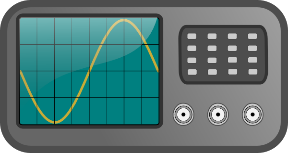
\includegraphics[width=0.1 \textwidth]{illustrations/scope}};
		\node[above right = of Chip] (PC) {
\includegraphics[width=0.1 \textwidth]{illustrations/pc}};
		\node[right = of Scope] (Trace) {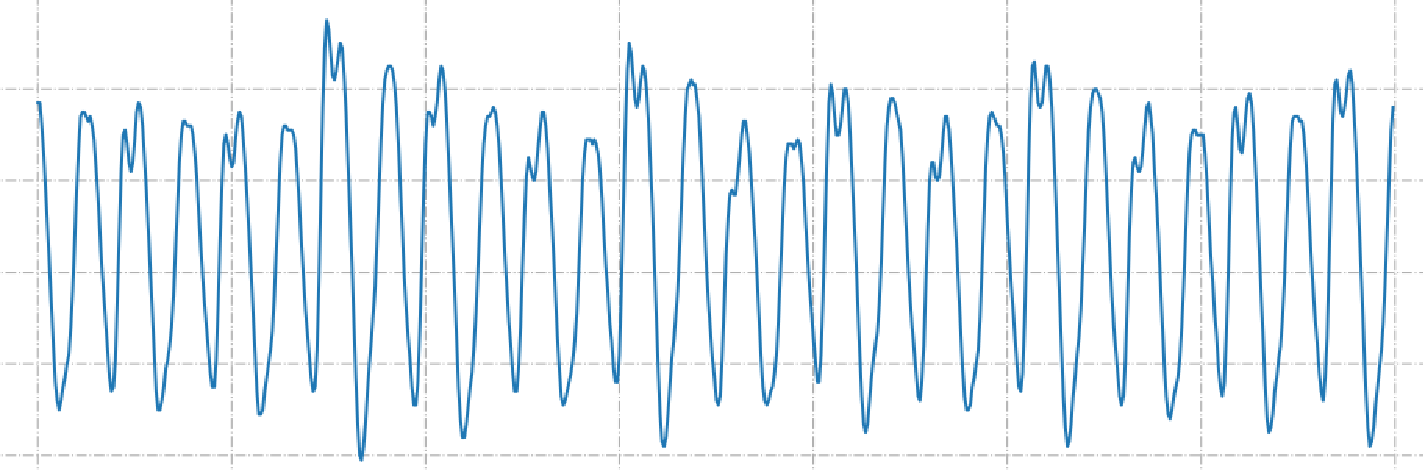
\includegraphics[width=0.2 \textwidth,angle=90]{illustrations/trace}\(\xxx\)};
		\node[rounded, fill=ceablue!30, right = of Trace] (Model) {\small \(\MLmodel(\xxx, \MLparam)\)};
		\node[right = of Model] (Scores) {
\includegraphics[width=0.2 \textwidth,angle=90]{illustrations/scores}};
		\node[rounded, fill=ceared!30, below = of Model] (Param) {\small Parameters \(\MLparam\)};
		\node[rounded, fill=ceadarkred!30, right = of PC] (Z) {\small \(\z = \miniEncrypt{\p, \keyTest}\)};


		\node[rounded, fill=cealime!30, right = of Scores] (Loss) {\small \(\lossFunc{\vNNOutput, \z}\)};

		\draw[->] (Chip)  -- (Scope);
		\draw[->] (Chip)  -- (PC);
		\draw[->] (Scope) -- (Trace);
		\draw[->] (PC)    -- (Z);
		\draw[->] (Trace) -- (Model);
		\draw[->] (Param) -- (Model);
		\draw[->] (Model) -- (Scores);

		\draw[->] (Scores) -- (Loss);
		\draw[->] (Z) -| (Loss);
		\draw[->] (Loss) |- (Param);
	\end{tikzpicture}
	\caption{Illustration of the workflow of the training of a \gls{dnn} in a profiled \gls{sca} context.}
	\label{fig:schema_dnn_sgd}
\end{figure}

Interestingly, the \gls{erm} principle introduced by the \gls{ml} framework remains a purely theoretical tool in most of the applications, and particularly in deep learning.
Indeed, it often cannot be implemented in practice, for several reasons that we will describe in the following subsections.
Finally, we explain in \autoref{sec:computing_gradient} how the derivatives of the loss function, a crucial element required by the optimization algorithm, is efficiently computed.
This description will serve as a discussion in \autoref{chap:gradient_viz}.


\subsection{\gls{sca} Metrics are Hard to Optimize}
\label{sec:erm_hard}
So far in this chapter, we have presented the \gls{ml} framework for a generic learning problem.
In particular, we have considered so far an abstract loss function \(\lossFunc{}\) to minimize, whose generic definition has been given in \autoref{eq:loss_function}.
It is indeed tempting at first sight to use the final performance metric as a loss function, in order to guarantee the convergence of the trained model towards the best possible one, according to \autoref{thm:consistency}.
Unfortunately, one cannot optimize with respect to any loss function, regardless the underlying hypothesis class \(\hypoclass\).

For example, in supervised classification the ultimate performance metric is the \emph{accuracy}, namely the rate of accurate predictions among the possible labels that may be recognized by the model.
% Definition
For any function \(\MLmodel: \leakSpace \rightarrow \realSet^{\card{\sensVarSet}}\), the accuracy is denoted by \(\acc_{\XXX, \Z}(\MLmodel)\) and is defined as:
\begin{equation}
	\acc_{\XXX, \Z}(\MLmodel) \eqdef \prob{\argmax_{\sensValue \in \sensVarSet}\MLmodel(\XXX)[s] = \Z} 
	 = \esper[\XXX, \Z]{\charac{\argmax_{\sensValue \in \sensVarSet}\MLmodel(\XXX)[s] = \Z}}
	\enspace .
\end{equation}
That is, this metric gives the rate of right predictions, or more precisely the probability that the highest score returned by a learning algorithm based on a single input data \(\XXX\) corresponds to the class \(\Z\) it is assigned.
Therefore, maximizing the accuracy is suitable to address the \emph{classification} task.

% NP-hard
Unfortunately, solving the \gls{erm} for \glspl{dnn} with the accuracy as a loss function turns out to be \gls{nph}~\cite[Sec.~20.5]{shalev-shwartz_understanding_2014}.
In a nutshell, the reason comes from the fact that the resulting training loss can be formulated as a sum of characteristic functions:%
\footnote{
	See \autoref{sec:notations} for a definition of a characteristic function.
}
\begin{equation}
	\acc_{\trainSet}(\MLmodel) \eqdef \frac{1}{\card{\trainSet}} \sum_{\xxx, \z \in \trainSet} \charac{\argmax_{\sensValue \in \sensVarSet}\MLmodel(\xxx)[s] = \z} \enspace .
	\label{eq:acc_charac}
\end{equation}
Each characteristic function in \autoref{eq:acc_charac} has null derivatives \gls{ae}, and so has the training loss of the accuracy, as depicted in \autoref{fig:example_acc} with the staged red curve depicting the training loss, as a sum of characteristic functions.
So gradient-descent-based optimization algorithms are useless, and no other efficient alternative could circumvent this issue.
\begin{figure}
	\centering
	\begin{tikzpicture}
		\begin{axis}[thick,axis x line=bottom, axis y line=left, no markers, xlabel = {\(\MLparam\)}, xtick=\empty, ytick=\empty, every axis x label/.style={at={(current axis.right of origin)}, anchor=north west}, legend pos=outer north east]
			\addplot[ceablue] {x^2};
			\addlegendentry{\(\LossFunc[\XXX, \Z]{\MLparam}\)}
			\addplot[samples=200, ceadarkred] {(round(2*x)/2)^2};
			\addlegendentry{\(\LossFunc[\trainSet]{\MLparam}\)}
		\end{axis}
	\end{tikzpicture}
	\caption{Toy example of a training loss made of characteristic functions with respect to a real valued learning parameter \(\MLparam\).
	Paradoxically, although the training loss \(\LossFunc[\trainSet]{\MLparam}\) has zero derivatives \gls{ae}, the generalization loss \(\LossFunc[\XXX, \Z]{\MLparam}\) may have non-null derivatives.}
	\label{fig:example_acc}
\end{figure}

% Classification -> SCA
Interestingly, this drawback also concerns the efficiency \(\MLmodel \mapsto \numTracesAttack(\MLmodel)\), defined in \autoref{sec:performance_metrics} as the minimal number of attack traces to succeed the attack beyond a probability threshold \(\beta\) fixed by the evaluator, and that we chose as an ultimate performance metric according to \autoref{final_task_prof}.
The corresponding training loss to minimize in the \gls{erm} would depend on the guessing vector defined in \autoref{eq:guess_vec}.
But the latter quantity is a sum of characteristic functions, hence meeting the same issues as the training loss corresponding to accuracy.
That is why the \gls{sca} metrics are hard to directly optimize.

% Other learning algorithms
More generally, this also holds for Random Forest and \glspl{svm}, two other learning algorithms used in the \gls{sca} literature~\cite{picek_curse_2019}: the former one is based on heuristics working reasonably well in practice~\cite[Chap.~18.2]{shalev-shwartz_understanding_2014} whereas the latter one must minimize another loss function called \emph{Hinge} loss~\cite[Chap.~15.2.3]{shalev-shwartz_understanding_2014}.

\subsection{The Need for a Surrogate Loss}
\label{sec:surrogate_loss}
The previous section raises the need for a suitable \emph{surrogate} loss function, either found among the usual functions considered in the \gls{dl} literature, or designed specifically for our problem.
In the literature, mostly two surrogate loss functions have been used in the \gls{sca} context: the \glsfirst{nll}~\cite{cagli_convolutional_2017,prouff_study_2018,kim_make_2019} and the \gls{mse}%
\footnote{
	From a purely optimization point of view, the \gls{mse} might suffer from problems~\cite{nielsen_neural_2018}.
	From a \gls{sca} evaluation point of view, the relevance of \gls{mse} is an open question~\cite{picek_bias_2019}, beyond the scope of this thesis.
}~\cite{maghrebi_breaking_2016, timon_non-profiled_2019,wegener_dlla_2019}.
Until a few years ago, nobody particularly raised the issue into the \gls{sca} community since the empirical results obtained for any loss function on several use cases got promising results from an attacker's point of view.
Nevertheless, from an evaluator's point-of-view, it remains necessary to assess whether the problem of minimizing the chosen training loss is actually equivalent to the profiled \gls{sca} optimization problem.
More precisely, whether:
\begin{enumerate}
	\item both problems share the same analytical optimal solution \(\MLmodel^\star\);
	\item improving a sub-optimal solution for one problem directly leads to get an improved sub-optimal solution for the other one.
\end{enumerate}
Tackling this issue is of great interest in \gls{sca}.
Indeed nowadays there might still be a gap between the recent practical successes of this class of attacks, and the theoretical soundness of \gls{dl}-based \gls{sca}: what is the sense of training a \gls{dnn} by minimizing a surrogate loss function from an \gls{sca} point of view?
This issue will be at the core of \autoref{chap:ches_20}.

\subsection{The Challenge of Optimization}
\label{sec:challenge_optimization}
We have seen that the interest of the surrogate loss function is to be differentiable with respect to all the learning parameters,%
\footnote{
	We recall that the parameters describing the architecture for which the loss is not differentiable are called \emph{\glspl{hp}}.
} 
in order to use a gradient based optimization algorithm such as \gls{sgd}.
Nevertheless, in \gls{dl}, this still raises an important issue, even when using a surrogate loss. 
Indeed, when considering the specific hypothesis class of \glspl{dnn}, the resulting \emph{objective}%
\footnote{
	The term ``objective'' function is the terminology used by the numerical optimization research community.
	It refers to the training loss function in the specific case of machine learning.
	In the following, we will rather use the term ``loss'' to design the function to minimize.
} 
function to optimize is shown to be highly non-convex~\cite{choromanska_loss_2015}, contrary to \glspl{svm} whose surrogate loss, \ie{} Hinge loss, spans a convex optimization problem.
Moreover, the solution to the problem is not unique: considering one \gls{dnn} model minimizing the training loss, the same model whose entries of the intermediate layers are permuted -- and so are the learning parameters accordingly -- would return the same result.
Hence, the number of equivalent solutions is \emph{combinatorial} with respect to the output size of the intermediate layers of the model.

As a consequence, the usual numerical optimization algorithms are not theoretically guaranteed to converge towards an optimal solution, which prevents the \gls{sgd} algorithm and its variants to perfectly instantiate the \gls{erm} principle.
In other words, the optimization error cannot be assumed to be negligible, as already discussed in \autoref{sec:erm_principle}.
Nevertheless, experience has surprisingly shown that those algorithms represent a satisfying heuristic~\cite{lecun_efficient_2012}, and the recent literature started to provide theoretical insights about this fact~\cite{du_gradient_2019,du_gradient2_2019}.

\subsection{Computing the Gradient}
\label{sec:computing_gradient}
So far in this section, we have explained that the \gls{erm} principle could be implemented by addressing a non-convex numerical optimization problem.
We explained in the previous sections to what extent perfectly solving this problem is hard in practice, although sound approximate solutions could be returned by an optimization algorithm such as the \gls{sgd}.
The latter algorithm -- and its variants -- rely on the computation of \emph{descent} directions based on the gradient of the loss function defined in \autoref{eq:empirical_loss} and computed with respect to the parameter vector, namely \(\grad[\MLparam]{\LossFunc[\trainSet]{\MLmodel(\cdot, \MLparam)}}\).
It is therefore of great interest to study to what extent providing the gradient of the loss function to the optimization algorithm is affordable when considering models from the hypothesis class of \glspl{dnn}.
This subsection is devoted to this discussion.
\begin{remark}
	The details provided in this subsection concern more generally any \gls{dl}-based problem, and not only \gls{sca}.
	Nevertheless, it will be useful for future discussions in \autoref{chap:gradient_viz}.
\end{remark}
The training loss to minimize being a sum of elementary losses over the profiling set, so is the gradient:
\begin{equation}
	\grad[\MLparam]{\LossFunc[\trainSet]{\MLmodel(\cdot, \MLparam)}} = 
	\frac{1}{\numTracesProf} \sum_{i=1}^{\numTracesProf} \grad[\MLparam]{\lossFunc{\MLmodel(\xxx_i, \MLparam), \z_i}} \enspace .
	\label{eq:grad_empirical_loss}
\end{equation}
It turns out that an algorithm called \emph{backward propagation} (\aka{} backprop) can exactly compute the gradient of \(\lossFunc{\MLmodel(\xxx_i, \MLparam), \z_i}\) with respect to \(\MLparam\) for roughly the same complexity of computing \(\lossFunc{\MLmodel(\xxx_i, \MLparam), \z_i}\) itself.
It relies on the use of the chaining rule recalled in \autoref{lemma:chaining_rule}.
Indeed, due to the layer-wise nature of \(\MLmodel(\cdot, \MLparam)\), the loss function, seen as a function of the parameter vector \(\MLparam\), can also be seen as a sequence of compositions of elementary functions whose derivatives can be computed in a closed-form solution.
Therefore, by using recursively the chaining rule on the given sequence of functions, one is able to exhibit an efficient procedure to exactly compute the gradient.

It is noticeable that for a composition of \(n > 2\) elementary functions, the chaining rule can be recursively applied in two manners, respectively denoted as \emph{forward} and \emph{reverse}.
We explain hereafter the stakes behind those two automatic differentiation modes on an example of compositions of \(n\) elementary functions \((f_i)_{1 \leq i \leq n}\) such that:
\begin{equation}
	f_i: \realSet^{m_{i-1}} \rightarrow \realSet^{m_i} \enspace ,
\end{equation}
where \(m_i \geq 1\) for \(0 \leq i \leq n-1\), \(m_{n-1} = \card{\sensVarSet}\), and \(m_n = 1\).
The resulting function to differentiate \(\ell: \realSet^{m_n}\rightarrow \realSet\) can then be written as:
\begin{equation}
	\lossFunc{\MLparam} = 
	\lefteqn{\overbrace{\phantom{f_n \circ \ldots \circ f_i}}^{\varphi_{n-i} \mbox{\tiny (Reverse)}}}
	f_n \circ \ldots \circ 
	\underbrace{f_i \circ \ldots \circ f_1}_{\psi_i \mbox{\tiny (Forward)}}
	\label{eq:autodiff_mode}
\end{equation}
We recall furthermore that the elementary functions \((f_i)_{1 \leq i \leq n}\) are assumed to be simple enough to derive closed-form expressions of their \glspl{jacob}.

% Forward mode
In a \emph{forward} mode, the chaining rule is applied from right to left%
\footnote{
	We draw the attention of the reader on the fact that when composing several functions, the notation \(f_2 \circ f_1\) must be read backward, hence ``forward'' means here ``right-to-left''.
} 
in \autoref{eq:autodiff_mode}.
That is, by considering the sequence of mappings defined by \(\psi_0 = I_d\) the identity mapping and \(\psi_{i+1} = f_{i+1} \circ \psi_i, \enspace 0 \leq i \leq n-1\), and by applying \autoref{lemma:chaining_rule}, it follows that:
\begin{equation}
	\underbrace{\jac{\psi_{i+1}}{\MLparam}}_{(m_{i+1}, m_0)} = \underbrace{\jac{f_i}{\psi_i(\MLparam)}}_{(m_{i+1}, m_i)} \cdot \underbrace{\jac{\psi_i}{\MLparam}}_{(m_i, m_0)}
	\label{eq:forward_mode}
\end{equation}
Since one remarks that \(\psi_n(\MLparam) = \lossFunc{\MLparam}\), it is then possible to compute its gradient by iteratively applying \autoref{eq:forward_mode}.
But this method requires to store the \glspl{jacob} of the mappings \(\psi_i\) whose sizes are respectively \(m_i \times m_0\), which might be prohibitive if the intermediate outputs are of high dimensionality.

% Reverse mode
In a \emph{reverse} mode, the chaining rule is applied from left to right in \autoref{eq:autodiff_mode}.
That is, by considering the sequence of mappings defined by \(\varphi_1 = f_n\) and \(\varphi_{i+1} = \varphi_i \circ f_{n-i}, \enspace 1 \leq i \leq n-1\), and by applying \autoref{lemma:chaining_rule}, it follows that for every \(\xxx \in \realSet^{m_{n-i}}\):
\begin{equation}
	\jac{\varphi_{i+1}}{\xxx} = 
	\jac{\varphi_i}{f_{n-i}(\xxx)} \cdot 
	\jac{f_{n-i}}{\xxx}
\end{equation}
By taking \(\xxx = \psi_{n-(i+1)}(\MLparam)\), it follows that:
\begin{equation}
	\underbrace{\jac{\varphi_{i+1}}{\psi_{n-(i+1)}(\MLparam)}}_{(1, m_{n-i})} = 
	\underbrace{\jac{\varphi_i}{\psi_{n-i}(\MLparam)}}_{(1, m_{n-i-1})} \cdot 
	\underbrace{\jac{f_{n-i}}{\psi_{n-(i+1)}(\MLparam)}}_{(m_{n-i-1}, m_{n-i})}
	\label{eq:reverse_mode}
\end{equation}
Since one remarks that \(\varphi_n = \ell\) it is here again possible to compute its gradient by iteratively applying \autoref{eq:reverse_mode}.
Yet, compared to the forward mode, two main differences should be noticed.
% First diff: need for a forward pass before differenciating
First, it is necessary to store all the intermediate computations \(\left(\psi_i(\MLparam)\right)_{1 \leq i \leq n}\) when previously computing the loss function \(\lossFunc{\MLparam}\), whereas in a forward mode the gradient can be directly computed without necessarily computing \(\lossFunc{\MLparam}\).
% Second diff: one only store 1 gradient instead of 1 jacobian matrix
Second, rather than storing a \gls{jacob} after each iteration, the reverse mode enables to only store a gradient of size \(m_{n-i}\), which is much lighter than in the forward mode.
That is why all the \glspl{api} devoted to \glspl{dnn} only use the reverse mode in their implementations, and are optimized in order to avoid the storage of any \gls{jacob}, hence the name of ``backprop'' which explicitly refers to the ``reverse'' mode.
This point will be later discussed in \autoref{chap:gradient_viz}.

% Biblio
The backprop algorithm has been independently discovered many times during the 70's and the 80's, in particular by Hinton \etal{} in 1986~\cite{rumelhart_learning_1986,hinton_backprop_1986}.
More generally, the backprop algorithm has paved the way towards \emph{automatic differentiation} which studies how to efficiently differentiate functions \emph{numerically},%
\footnote{
	\ie{} in opposition to \emph{symbolic} differentiation considering only algebraic formulations of a function.
} 
which is often crucial in machine learning.
The interested reader may refer to the survey of Baydin \etal{}~\cite{baydin_automatic_2017}.

\subsection{Some \glspl{api}}
\label{sec:apis}
Training \glspl{dnn} with optimization algorithms is nothing but linear algebra computations -- \eg{} scalar and matrix product -- in very high dimensionality, typically \(10^5 - 10^6\).
To scale with this range, the implementation must leverage massively parallel programming, either in \gls{cpu} clusters of on \glspl{gpu}.
That is why until few years ago, the \gls{ml} practitioners used to need strong skills in a broad spectrum of programming fields.
Those skills were hard to gather into a research team, and most of the time of researchers was devoted to implementing models which were not easily reproducible by the scientific community.

% APIs in Deep Learning
That is why, with the emergence of deep learning in the beginning of the 2010's, several \glspl{api} have been released by the machine learning community.
Although the very first public library \textsf{Theano}~\cite{theano} is not maintained anymore by its authors, several other \glspl{api} have been publicly developed over the last few years, such as \textsf{Pytorch}~\cite{pytorch_2019}, supported by Facebook; \textsf{Tensorflow}~\cite{tensorflow2015-whitepaper}, supported by Google; or \textsf{Keras}~\cite{chollet2015keras}, an extension of \textsf{Tensorflow} initiated by Chollet.
In particular, the source code developed for this thesis has been written in \textsf{Python} with the help of the \textsf{Pytorch} \gls{api},%
\footnote{The library is available at \url{pytorch.org}.}
and is run on a workstation with a \textsf{Nvidia Quadro M4000} \gls{gpu} with 8 GB memory and 1664 cores, and 32~GB of \gls{ram}.

\subsection{On the Accuracy as a Monitoring Metric}
\label{sec:issue_accuracy}
We have seen in \autoref{sec:erm_hard} that in supervised classification, it is not possible to directly maximize the accuracy of \glspl{dnn}, since it is a \gls{nph} problem.
Despite its impossibility to directly minimize, most of the works considering \gls{dl}-based \gls{sca} made use, explicitly or implicitly, of the accuracy as a monitoring metric, assuming that such a performance measure may still be informative of the quality of a trained model.

Cagli \etal{}~\cite{cagli_convolutional_2017} and Picek \etal{}~\cite{picek_curse_2019} were the first to raise this issue, namely the relevance of the \emph{accuracy}, a widely used \gls{ml} performance metric, in the context of \gls{sca}.
Unfortunately, we explain hereafter that it is not the case.

It turns out that the optimal model for \gls{sca}, which is \(\MLmodel^{\star} = \prob{\Z \given \XXX}\), is also the optimal classifier for the supervised classification task.%
\footnote{
	The \gls{ml} literature often uses the term \emph{Bayes' classifier} to denote the optimal classifier for the classification task.
} 
This means that for any function \(\MLmodel: \leakSpace \rightarrow \probSet{\sensVarSet}\) we have:
\begin{equation}
	\acc(\MLmodel) \leq \acc(\MLmodel^{\star}) \enspace .
\end{equation}
In other words, both supervised classification problem and \autoref{final_task_prof} share the same analytical optimal solution \(\MLmodel^\star\), which is the first of the two conditions stated in \autoref{sec:surrogate_loss} to get a loss function equivalent to our \gls{sca} efficiency metric.
Thus, the accuracy might be a good metric candidate.
Yet, both problems sharing the same optimal solution \(\MLmodel^\star\) does not necessarily mean that they are equivalent, since it remains to verify that improving sub-optimal solutions for one problem should lead to improved sub-optimal solutions for the other.

Cagli \etal{}\,recalled that the accuracy could be translated into another \gls{sca} metric, namely the success rate when recovering the key with one trace \(\succRate(1)\).
In a sense, \(\acc(\MLmodel)\) is the \emph{dual} metric of \(\numTracesAttack(\MLmodel, 1, \beta)\): the former one fixes \(\numTracesAttack=1\) and estimates the corresponding threshold \(\beta\), whereas the latter one fixes the threshold and estimates the minimum value \(\numTracesAttack\) such that \(\succRate(\numTracesAttack, \MLMLEscore{\attackSet}{\MLmodel}, 1) \geq \beta\) -- see \autoref{eq:SR}.
Cagli \etal{}\,have emphasized that although this could have a sense in some specific scenarios, \eg{}, when evaluating implementations of asymmetric cryptographic primitives, this does not necessarily have a sense to evaluate the robustness of a target against an attack involving only one trace.
That is why at first sight, accuracy does not seem appropriate in our context.

Picek \etal{} empirically confirmed a similar observation at \textsc{Ches}'19~\cite{picek_curse_2019}.
For several learning algorithms, such as \glspl{svm} and Random Forests, they empirically compared the obtained \gls{ge} with the accuracy, and they found out that there is no clear link between them.
More precisely, they argue that a high accuracy -- \ie{}, with respect to the one obtained with a model providing completely random predictions -- is a clue for effective attacks, though the inverse does not empirically hold: a low accuracy does not necessarily imply a failed key recovery.
However, the latter case may often happen, especially with protected implementations where the noise artificially induced by the counter-measures reduces the performances of the optimal model, and so the accuracy.

As a conclusion to the two latter sections, the accuracy is not only useless for the implementation of the \gls{erm}, as already concluded in the end of \autoref{sec:erm_hard}, but is also a poor metric to monitor in an \gls{sca} context.
Recently, new ways to monitor the quality of a \gls{dnn} have been proposed, in particular by Robissout \etal{}~\cite{robissout_online_2020} and Perin \etal{}~\cite{perin_learning_2020}.
Although this brings new insights, those monitoring metrics partially circumvent the problems raised by the accuracy, since the metrics proposed there are not optimizable.
Finding a proper loss function which is useful not only as a quantity to optimize but also as a metric to monitor is the core problem which will be addressed in \autoref{chap:ches_20}.

\section{An Overview of the Literature}
    \label{sec:review_dl_sca}
    %%%%%%%%%%%%%%%%%%%%%%%%%%%%%%%%%%%%%%%%%%%%%%%%%%%%%%%%%%%%%%%%%%%%%%%%%%%%%%%%
%                       REVIEW DEEP LEARNING FOR SCA                           %
%%%%%%%%%%%%%%%%%%%%%%%%%%%%%%%%%%%%%%%%%%%%%%%%%%%%%%%%%%%%%%%%%%%%%%%%%%%%%%%%
The past few years have seen the emergence of contributions on \gls{sca} using more and more \gls{dl} techniques.
The community committed to investigate several models leading to practical attacks against several implementations. 
The very first works came from Martinasek \etal{}~\cite{martinasek_innovative_2013,martinasek_profiling_2016}, Gilmore \etal{}~\cite{gilmore_neural_2015}, whereas other \gls{ml} techniques have been investigated by Heuser \etal{}~\cite{heuser_intelligent_2012} and Lerman \etal~\cite{lerman_power_2014,lerman_machine_2015}.
Hereafter, we focus on the specific use of \gls{dl} rather than on other \gls{ml} algorithms.
The reader interested in a complete review of the use of every learning algorithm in \gls{sca} may refer to the comprehensive survey of Hettwer \etal{}~\cite{hettwer_applications_2020}.

% Target Primitives
The \gls{asym_crypto} has been by now investigated by Carbone \etal{} concerning the \gls{rsa} primitive~\cite{carbone_deep_2019}, and by Weissbart \etal{}~\cite{weissbart_one_2019} concerning elliptic curves.
In both works, results are as promising as for the symmetric context.

Auto-Encoders appeared as a valid solution to perform dimensionality reduction and pre-processing of side-channel signals~\cite{maghrebi_breaking_2016}. 
The temporal aspect of side-channel traces leads the community to explore as well some recurrent neural network structures, in particular the \gls{lstm} one~\cite{maghrebi_deep_2019}.
\glspl{cnn} appeared more suitable in presence of signal desynchronization, and thus in presence of counter-measures injecting desynchronization in signals~\cite{cagli_convolutional_2017,prouff_study_2018,kim_make_2019}.

\subsection{Unsupervised Learning for \gls{sca}}
Moreover one may remark that the great majority of works apply deep learning to perform profiling attacks, and logically exploits for the learning algorithm a supervised experience.
A very few works proposed a non-profiling deep-learning-based attack.
First, Timon proposed at \textsc{Ches}'19~\cite{timon_non-profiled_2019} an extension of the \gls{lra} attack~\cite{schindler_stochastic_2005}.
However, this means that the learning algorithm still exploits a supervised experience, in which labels are assigned according to different key hypotheses.

Second, Ramezanpour \etal{}~\cite{ramezanpour_scaul_2020} extended the works of Timon in several ways, by using \glspl{lstm} as an unsupervised feature extractor, and by using some analysis developed by Wang \etal{}~\cite{wang_ridge_2018} as a leakage modeling method.

A full-non-supervised track, based for example onto deep clustering techniques recently proposed in the computer vision domain, is still unexplored in the side-channel context.

\subsection{Exploring the \gls{dl} Strategies for \gls{sca}}
This vast panorama of experimentally investigated tools have subsequently emphasized the need for a deep understanding of their architectural properties.  
A well-established methodology -- beyond those already proposed~\cite{prouff_study_2018,zaid_methodology_2019} -- to tune the (very) high number of \glspl{hp} in these models would be very useful.
Furthermore, since in ML the learning algorithms are driven by data, the data management is a crucial point and related issues and good practices have been investigated in this sense.
Cagli \etal{}~\cite{cagli_convolutional_2017} and Kim \etal{}~\cite{kim_make_2019} proposed data augmentation techniques to control and decrease the estimation error~\eqref{eq:err_est}.
But many questions about the utility and /or necessity of performing some pre-processing like dimensionality reduction~\cite{maghrebi_deep_2019}, realignment~\cite{cagli_convolutional_2017,zhou_deep_2019}, de-noising~\cite{wu_remove_2019}, under/over-sampling to deal with class imbalance~\cite{picek_curse_2019}, or the conversion of data into the frequency domain by means of Fourier or Wavelets transforms~\cite{yang_convolutional_2018,destouet_wavelet_2020} have been raised.

\subsection{Support for Understanding}
Although \glspl{dnn} show encouraging results in an evaluation context of \gls{sca}, following the recent hype of deep learning in pattern recognition, many people in the community remain skeptical and reluctant to this approach.
This is mostly due to the \emph{black-box}%
\footnote{
    This terminology shall not be confound with the same term used for black-box attack scenarios discussed in \autoref{chap:sca}.
} 
aspect of those algorithms, \ie{} the fact that they do not provide any insight about how the informative leakage occurs in the \gls{sca} traces.
Although not of great interest for the attackers whose ultimate goal is only to recover the secret key, this represents a huge stake for evaluators and developers.

To provide understanding in \gls{dl} models behavior, a track of recent works -- including ours -- proposed the use of some visualization techniques, with the threefold intent of characterizing the sensitive leaking part of the side-channel traces, understanding the nature of the signal information that a given neural network is able or not to exploit~\cite{masure_gradient_2019,hettwer_deep_2019,timon_non-profiled_2019,vanDerValk_kilroy_2019} and validating the \glspl{hp} choices~\cite{zaid_methodology_2019}.
Furthermore, visualization techniques aiming at focusing on \gls{dl} in order to help tuning their \glspl{hp} or understanding their prediction is a long running challenge in the visualization and machine learning community~\cite{hohman_visual_2019,garcia_task_2018}.
This issue will be the core discussion of \autoref{chap:gradient_viz}.

\subsection{\gls{dl}-based \gls{sca} and Counter-Measures}
The community already wondered about the efficiency of existing side-channel counter-measures against \gls{dl}-based \gls{sca}. 
Many works -- including ours -- recently investigated the robustness of classic counter-measures, in particular the high-order secret-sharing~\cite{maghrebi_breaking_2016,prouff_study_2018,kim_make_2019,timon_non-profiled_2019,maghrebi_deep_2019,masure_comprehensive_2019,zhou_deep_2019,bronchain_dissection_2020}.
The \gls{dl}-based \gls{sca} showed very fast outperforming results with respect to the previous state-of-the-art attacks.
The main advantage of \gls{dl}, compared to regular \gls{sca} attacks is that \gls{dl} is not technically limited by the minimal number of points which must be jointly processed, which was originally one of the strong practical arguments to use high-order secret-sharing, as we argued in \autoref{sec:masking}.
Nevertheless, Bronchain \etal{} recently emphasized a use case where automated attacks with \gls{dl} did not succeed against a software target protected with affine secret-sharing whereas classical template attacks involving a subtle dissection of the open source code~\cite{bronchain_dissection_2020}.
This lets one think that \gls{dl}-based \gls{sca} could not always represent a better approach than classical Gaussian templates.
We further discuss this case in the perspectives presented in the global conclusion of this thesis.


This also raises the challenge of knowing exactly the necessary number of traces for the training phase of a \gls{dl} model -- \ie{} the sample complexity, and how secret-sharing could have an impact on this constraint. 
Until now, only Picek \etal{} started tackling the question~\cite{picek_profiling_2019}. 

In addition, to the best of our knowledge, no sound counter-measure has been exhibited so far in the literature to specifically counteract deep learning techniques in side-channel analysis.
Nevertheless, it seems that perturbing the inputs or adding dummy operations to fool a network could help developers in the protection of their implementation against deep learning attackers~\cite{bertrand_fool_2020}.

\subsection{Multi-Task Learning}
\label{sec:multi-task}
Some works make the hypothesis that several sensitive variables, processed in a similar way by the device during the cryptographic algorithm execution, may be targeted while keeping unchanged the neural network architecture (\ie{} the \glspl{hp} are tuned only once)~\cite{green_not_2019}.
A similar approach has been proposed by Wang \etal{}~\cite{wang_tandem_2020}, who combined the predictions of three different models targeting three different sensitive intermediate computations in an \gls{fpga} implementation of \gls{aes}.
A recent work from Maghrebi~\cite{maghrebi_deep_2020} leverages this finding by proposing to solve the \gls{sca} problem with a single multi-labeling classifier.
However, his solution, as is, is limited to learning only two labels at the same time.
In the general conclusion of this thesis, we will further discuss this new line of work.

The multiple classifier concept is analogously proposed in~\cite{destouet_wavelet_2020}, where several overlapping modelizations of a sensitive variable are independently recognized by several classifiers whose outputs are jointly exploited in the attack phase.
In addition to these multiple outputs, it has been observed that training a deep neural network in a multi-task fashion results in having the performances of each single classifier increased.

\subsection{Multi-Sources}
The multi-source idea to enrich signal databases, meaning harvesting at the same time several side-channel signals (for example power consumption and \gls{em} irradiation captured with multiple probes placed nearby different areas of the device) and exploiting them synergistically, has been explored by Genevey-Metat \etal{} at \textsc{C\&esar} 2019~\cite{genevey_combining_2019}.
Furthermore, learning with multiple and even heterogeneous sources remains an open topic in the machine learning community.

\subsection{Portability}
As a related topic, Carbone \etal{}~\cite{carbone_deep_2019} and Bhasin \etal{}~\cite{bhasin_mind_2019} tackled the portability issue: these works aim to understand the performance effects observed on \gls{dl} models while conducting a profiling phase on a device which may not be a perfect clone of the target, in opposition to what is assumed throughout this thesis.

\section{Conclusion}
    The machine learning framework enables to extend the leakage modelization in a profiling attack scenario to much more powerful hypothesis classes, which has been at the origin of new recent milestones in \gls{sca}.
    Nevertheless, in view of the current state of the art, we are today in an uncomfortable situation.
    Indeed, the replacement of the Profiled \gls{sca} Optimization Problem -- \ie{} \autoref{final_task_prof}, so far tackled classical profiling attacks such as \glspl{gta}, by the Supervised Classification Problem -- \ie{} finding a model maximizing the accuracy defined by \autoref{eq:acc_charac}, thanks to \glspl{dnn}, shows promising efficiency gains.
    Nevertheless, several recent papers question the theoretical soundness of the latter problem substitution~\cite{cagli_convolutional_2017,picek_curse_2019}.
    This situation prevents the \gls{sca} community to get a clear picture of the potential impact of \gls{ml} and \gls{dl}, especially from the developers' perspective.
    Indeed, though an attacker only needs to know an efficient practical approach to train a \gls{dnn}, a developer needs a theoretically grounded approach to be able to give the best security bounds on the complexity of mounting a profiling attack, especially when the implementation is protected by counter-measures.

    More specifically, through the review of the deep learning approach and the literature review, we have emphasized several caveats which should be addressed by the \gls{sca} community:
    \begin{itemize}
        \item How can one prove that the underlying optimization problem materializing the training phase is a theoretically sound approach for \autoref{final_task_prof}, beyond the recent empirical success?
        This requires to address the issue of choice of the loss function, and the study of the optimization error yield by the \gls{sgd} or its variants.
        \item How far can deep learning go to approximate the true leakage model, even in presence of counter-measures?
        Said equivalently, is there any sound \gls{dl}-oriented counter-measure which could protect the implementations of cryptographic primitives against this threat?
        \item How can an evaluator get a clear understanding of what happens during the profiling phase with \glspl{dnn}, in order to draw a fair diagnosis of the device under evaluation?
    \end{itemize}
    Our work in the remaining of this thesis aims at grounding the use of \glspl{dnn} in the \gls{sca} context, by addressing those issues in the next three chapters.